\documentclass[11pt]{article}

\usepackage{amssymb,amsmath,amsfonts,booktabs,eurosym,float,geometry,ulem,graphicx,caption,color,setspace,sectsty,comment,footmisc,caption,pdflscape,subfigure,array,makecell}

% \usepackage[authoryear]{natbib}
\usepackage[round,authoryear]{natbib}
% \bibliographystyle{plainnat}
\usepackage[colorlinks=true,linkcolor=blue,citecolor=blue,urlcolor=blue]{hyperref}

\usepackage{bm}
\usepackage{xcolor}
\newcommand{\todo}[1]{\textcolor{red}{[TODO: #1]}}

\normalem
\onehalfspacing
\newtheorem{theorem}{Theorem}
\newtheorem{corollary}[theorem]{Corollary}
\newtheorem{proposition}{Proposition}
\newenvironment{proof}[1][Proof]{\noindent\textbf{#1.} }{\ \rule{0.5em}{0.5em}}

\newtheorem{hyp}{Hypothesis}
\newtheorem{subhyp}{Hypothesis}[hyp]
\renewcommand{\thesubhyp}{\thehyp\alph{subhyp}}
\newcolumntype{L}[1]{>{\raggedright\let\newline\\arraybackslash\hspace{0pt}}m{#1}}
\newcolumntype{C}[1]{>{\centering\let\newline\\arraybackslash\hspace{0pt}}m{#1}}
\newcolumntype{R}[1]{>{\raggedleft\let\newline\\arraybackslash\hspace{0pt}}m{#1}}
\geometry{left=0.8in,right=0.8in,top=1.0in,bottom=1.0in}

\begin{document}

\begin{titlepage}
\title{Robust Pricing Kernel Estimation for Bitcoin Options under the SVCJ Model}%\thanks{This paper is supported by the National Science and Technology Council of Taiwan under Grant No. 112-2118-M-A49-001-MY2; the Higher Education Sprout Project of the Ministry of Education of Taiwan, ROC.}%
\author{Huei-Wen Teng\thanks{Department of Information Management and Finance, National Yang Ming Chiao Tung University. Email: \href{mailto:hwteng@nycu.edu.tw}{hwteng@nycu.edu.tw}} \and Chin Hsu\thanks{Department of Applied Mathematics, National Yang Ming Chiao Tung University. Email: \href{mailto:hc330.sc14@nycu.edu.tw}{hc330.sc14@nycu.edu.tw}}  \and Wolfgang Haerdle}
\date{\today}
\maketitle

\begin{abstract}
\noindent 
The pricing kernel — the stochastic discount factor linking risk and return across all states of the world — simultaneously determines fair derivative prices, risk premia magnitudes, and optimal hedge ratios, making it the central object of modern asset pricing. For Bitcoin, the world's largest cryptocurrency with a derivatives market exceeding \$40 billion in open interest, its shape and dynamics remain largely uncharacterized. Existing Bitcoin option pricing studies operate under either the physical measure or the risk-neutral measure in isolation, and no study has yet imposed a unified Stochastic Volatility with Correlated Jumps (SVCJ) framework simultaneously across both measures, leaving recovered pricing kernels internally inconsistent and the Bitcoin pricing kernel puzzle unresolved. This thesis estimates both measures within a common SVCJ specification — the physical measure via rolling MCMC on spot returns and the risk-neutral measure via daily Levenberg–Marquardt calibration on Deribit options — recovering the pricing kernel as an internally consistent density ratio and deploying it as a trading signal to test whether Bitcoin pricing kernel anomalies are economically exploitable. The study covers January 2020 to December 2024, using daily Bitcoin spot returns and a comprehensive panel of European-style inverse options across multiple strikes and maturities from Deribit. The analysis proceeds through four stages: rolling MCMC estimation under $\mathbb{P}$
, daily calibration under $\mathbb{Q}$
, nonparametric pricing kernel estimation with monotonicity tests, and backtesting of a Variance Risk Premium-filtered delta-hedged short straddle strategy.
\vspace{0in}\\
\noindent\textbf{Keywords:} Bitcoin, pricing kernels, stochastic discount factor, stochastic volatility with correlated jumps, cryptocurrency derivatives\\
\vspace{0in}\\
\noindent\textbf{JEL Codes:} JEL1, JEL2, JEL3\\

\bigskip
\end{abstract}

\setcounter{page}{0}
\thispagestyle{empty}
\end{titlepage}

\doublespacing
%\tableofcontents
%\listoftables
%\listoffigures
%\clearpage

\section{Introduction}

Bitcoin has evolved from a largely retail and exchange-specific trading venue into a globally traded asset held, intermediated, and hedged through increasingly institutional channels. The approval and subsequent trading of spot Bitcoin exchange-traded products have made Bitcoin exposure accessible through conventional portfolio infrastructure, while the development of liquid listed and over-the-counter option markets has created a cross-section of prices that embeds forward-looking assessments of volatility, jump risk, and tail-state compensation. Yet the economic object implied by these option prices remains only partially understood. Bitcoin is traded continuously across venues and jurisdictions, and its return dynamics display precisely the features that make standard asset-pricing restrictions difficult to impose: strong non-Gaussianity, heavy tails, abrupt price discontinuities, volatility clustering, and recurrent regime shifts. In such an environment, neither a representative-agent Euler equation estimated from low-frequency consumption data nor a lognormal diffusion calibrated to a single volatility parameter is likely to provide a satisfactory account of how investors value Bitcoin payoffs.

{\color{red}This paper studies Bitcoin option prices through the lens of the pricing kernel. For a payoff $\psi(S_T)$ written on the terminal Bitcoin price $S_T$, no-arbitrage valuation gives
\begin{equation}
P_t=E_t^\mathbb{Q}\left[e^{-r\tau}\psi(S_T)\right]
    =E_t^\mathbb{P}\left[e^{-r\tau}K_t(S_T)\psi(S_T)\right],
\end{equation}
where $\mathbb{P}$ is the physical measure, $\mathbb{Q}$ is the risk-neutral measure, $\tau=T-t$, and
\begin{equation}    
K_t(x)=\frac{q_t(x)}{p_t(x)}
\end{equation}
is the ratio of the risk-neutral density to the physical density.} This object is central because it converts statistical probabilities into state prices. A dollar paid in a state with high marginal value should command a larger state price than a dollar paid in a state with low marginal value; consequently, the shape of $K_t$ summarizes how the market prices downside risk, upside speculation, variance risk, and jump risk. The pricing-kernel representation also makes clear why Bitcoin options are an informative laboratory: the same terminal distribution may receive very different physical and risk-neutral weights when investors demand compensation for crash risk or for volatility-jump exposure.

The classical stochastic-discount-factor literature provides the first benchmark for this problem. \citet{HansenSingleton1982} estimate Euler-equation restrictions by generalized method of moments, showing how asset returns can discipline intertemporal marginal rates of substitution. Hansen and Jagannathan \citep{HansenJagannathan1991} derive volatility bounds for admissible stochastic discount factors, thereby turning asset-return data into a diagnostic restriction on pricing models. These approaches are foundational, but they are not directly tailored to Bitcoin. Euler-equation estimation requires specifying preferences and information variables, often relying on consumption or macroeconomic data that are difficult to interpret for a globally traded cryptoasset. Hansen--Jagannathan bounds are powerful diagnostics, but they do not by themselves recover the state-by-state pricing kernel embedded in option prices. Our setting therefore calls for an option-based approach that can recover the relative valuation of future Bitcoin states more directly.

A parallel option-based literature exploits the fact that option prices reveal state prices. Breeden and Litzenberger \citep{BreedenLitzenberger1978} show that the second derivative of call prices with respect to strike identifies state-contingent prices. Building on this insight, Shimko \citep{Shimko1993} smooths implied volatility before recovering the risk-neutral density, while A{\"i}t-Sahalia and Lo \citep{AitSahaliaLo1998} develop a nonparametric estimator of state-price densities implicit in option prices. A{\"i}t-Sahalia and Lo \citep{AitSahaliaLo2000} further combine option-implied state prices with estimates of the physical distribution to infer implied risk aversion. These studies formalize the empirical density-ratio logic underlying this paper: once the physical density $p_t$ and risk-neutral density $q_t$ are estimated for the same horizon and state variable, their ratio gives an empirical pricing kernel. In practice, however, both densities are difficult to estimate. Risk-neutral density recovery is a continuous-strike identification result applied to discrete, noisy, maturity-specific option data; physical density estimation is sensitive to the historical window, tail observations, and the assumed return dynamics. These difficulties are especially acute for Bitcoin, where tail states are economically central rather than peripheral.

The empirical pricing-kernel literature also warns that naively estimated density ratios can produce economically puzzling shapes. Jackwerth \citep{Jackwerth2000} and A{\"i}t-Sahalia and Lo \citep{AitSahaliaLo2000} document pricing kernels that are locally increasing over parts of the state space, a finding commonly referred to as the pricing-kernel puzzle because it appears inconsistent with a globally decreasing marginal utility schedule. Rosenberg and Engle \citep{RosenbergEngle2002} estimate empirical pricing kernels using flexible physical densities and parametric restrictions on the kernel, emphasizing the role of the physical return model in shaping the density ratio. Christoffersen, Heston, and Jacobs \citep{ChristoffersenHestonJacobs2013} show that option anomalies can be captured by a variance-dependent pricing kernel, while Linn, Shive, and Shumway \citep{LinnShiveShumway2018} argue that conditioning and information-set mismatch are central to understanding option-implied stochastic discount factors. These contributions imply that a Bitcoin pricing kernel should not be estimated as an unconditional object averaged across market regimes. It should be conditional on the current volatility state, option-implied distribution, and market environment.

The Bitcoin setting sharpens these econometric and economic issues. First, the physical density is difficult to estimate. Historical kernel density estimators are flexible but fragile in the tails; GARCH-type models capture volatility clustering but typically handle jumps only indirectly; and purely diffusion-based stochastic-volatility models can understate discontinuities in returns and volatility. Second, the risk-neutral density is also difficult to recover. Breeden--Litzenberger identification requires a smooth continuum of strikes, whereas observed Bitcoin options are discrete, liquidity-constrained, and unevenly distributed across moneyness and maturities. Nonparametric smoothing of the implied-volatility surface reduces noise but introduces bandwidth, interpolation, extrapolation, and no-arbitrage choices. Third, the density-ratio construction magnifies errors: small mistakes in either $p_t$ or $q_t$ can become economically large when $q_t/p_t$ is evaluated in the tails. These concerns motivate a model that is sufficiently structured to stabilize tail inference, but sufficiently rich to match the discontinuous and heteroskedastic nature of Bitcoin returns.

We therefore estimate Bitcoin pricing kernels under the stochastic volatility with correlated jumps (SVCJ) model. The SVCJ framework extends stochastic-volatility models by allowing both the return and variance processes to jump, with contemporaneous dependence between return-jump and volatility-jump sizes. This feature is economically important for Bitcoin: large negative returns often coincide with abrupt increases in uncertainty, and option prices should reflect compensation not only for diffusive variance risk but also for jump-arrival risk and co-jump risk. Our model builds on the jump-diffusion and stochastic-volatility option-pricing literature, including Merton \citep{Merton1976}, Heston \citep{Heston1993}, Duffie, Pan, and Singleton \citep{DuffiePanSingleton2000}, and Eraker, Johannes, and Polson \citep{ErakerJohannesPolson2003}. Recent cryptocurrency-option studies similarly emphasize that Bitcoin option prices require models with stochastic volatility, jumps, and co-jumps \citep{HouWangChenHaerdle2020,MaticPackhamHaerdle2021}. Relative to these studies, our focus is not only on option valuation, but also on the state-price implications of the model through the pricing kernel.

Our empirical design uses historical Bitcoin returns to estimate the physical distribution and Deribit Bitcoin options to estimate the risk-neutral distribution, imposing the same SVCJ structure under both measures. This common dynamic structure is important. It allows differences between $P$ and $Q$ to be interpreted as compensation for variance risk, jump risk, and return-volatility co-jump risk rather than as artifacts of using unrelated density estimators. It also allows the pricing kernel to be conditional: for each estimation date and maturity, the kernel is tied to the prevailing level of volatility, the calibrated option surface, and the current state of the Bitcoin market. In contrast to an unconditional density ratio that averages across market regimes, our approach is designed to ask whether Bitcoin state prices behave differently during calm, speculative, and stress periods.

This paper makes three contributions. First, it contributes to the empirical pricing-kernel literature by constructing a robust, conditional pricing kernel for a nontraditional asset whose trading calendar, investor base, and tail behavior differ sharply from equity-index markets. Second, it contributes to cryptocurrency option pricing by using a unified SVCJ framework to compare the physical and risk-neutral laws of Bitcoin, thereby quantifying variance, jump, and co-jump risk premia embedded in option prices. Third, it contributes to the literature on the pricing-kernel puzzle by examining whether the nonmonotonicities documented in index-option markets also arise in Bitcoin, and whether they are robust to a model that explicitly accounts for stochastic volatility and correlated jumps. Recent evidence suggests that Bitcoin risk premia are state-dependent and that Bitcoin pricing kernels can exhibit pronounced nonlinear shapes \citep{AlmeidaGrithMiftachovWang2024}; our framework provides a structural way to study these patterns through the separate channels of diffusive volatility, jump intensity, and jump-size dependence.

The rest of the paper proceeds as follows. Section~2 introduces data. Section~3 introduces the SVCJ model under the physical and risk-neutral measures. Section~4 describes the Bitcoin return and option data and the estimation strategy. Section~5 presents the estimated physical and risk-neutral distributions, the resulting pricing kernels, and robustness checks across maturities and market regimes. Section~6 discusses implications for Bitcoin risk premia, option valuation, and portfolio allocation. Section~7 concludes.



%\subsection{Organization of this paper}



\section{Data} \label{sec:data}
This study employs two complementary datasets covering the period from January 1, 2020 to December 31, 2024: daily Bitcoin spot prices for physical measure estimation and intraday Deribit BTC inverse option transaction records for risk-neutral measure calibration. The analysis presented here focuses on the 2024 subsample for illustrative purposes, as it encompasses the most liquid and eventful period in the sample.\todo{To be determined what period(2020$\sim$2024 or only 2024) to show}

\subsection{Bitcoin Spot Prices and Log Returns}
Bitcoin spot prices are sourced at daily frequency and exhibit a pronounced bull market throughout 2024, rising from approximately \$40,000 at the start of the year to a peak exceeding \$106,000 in late November before retracing to approximately \$93,000 by year-end (Figure 1, left panel). This appreciation was driven by two structural catalysts: the approval of spot Bitcoin ETFs in the United States in January 2024 and the fourth Bitcoin block reward halving in April 2024, both of which materially shifted the supply-demand balance and attracted substantial institutional inflows.

\begin{figure}[h]
    \centering
    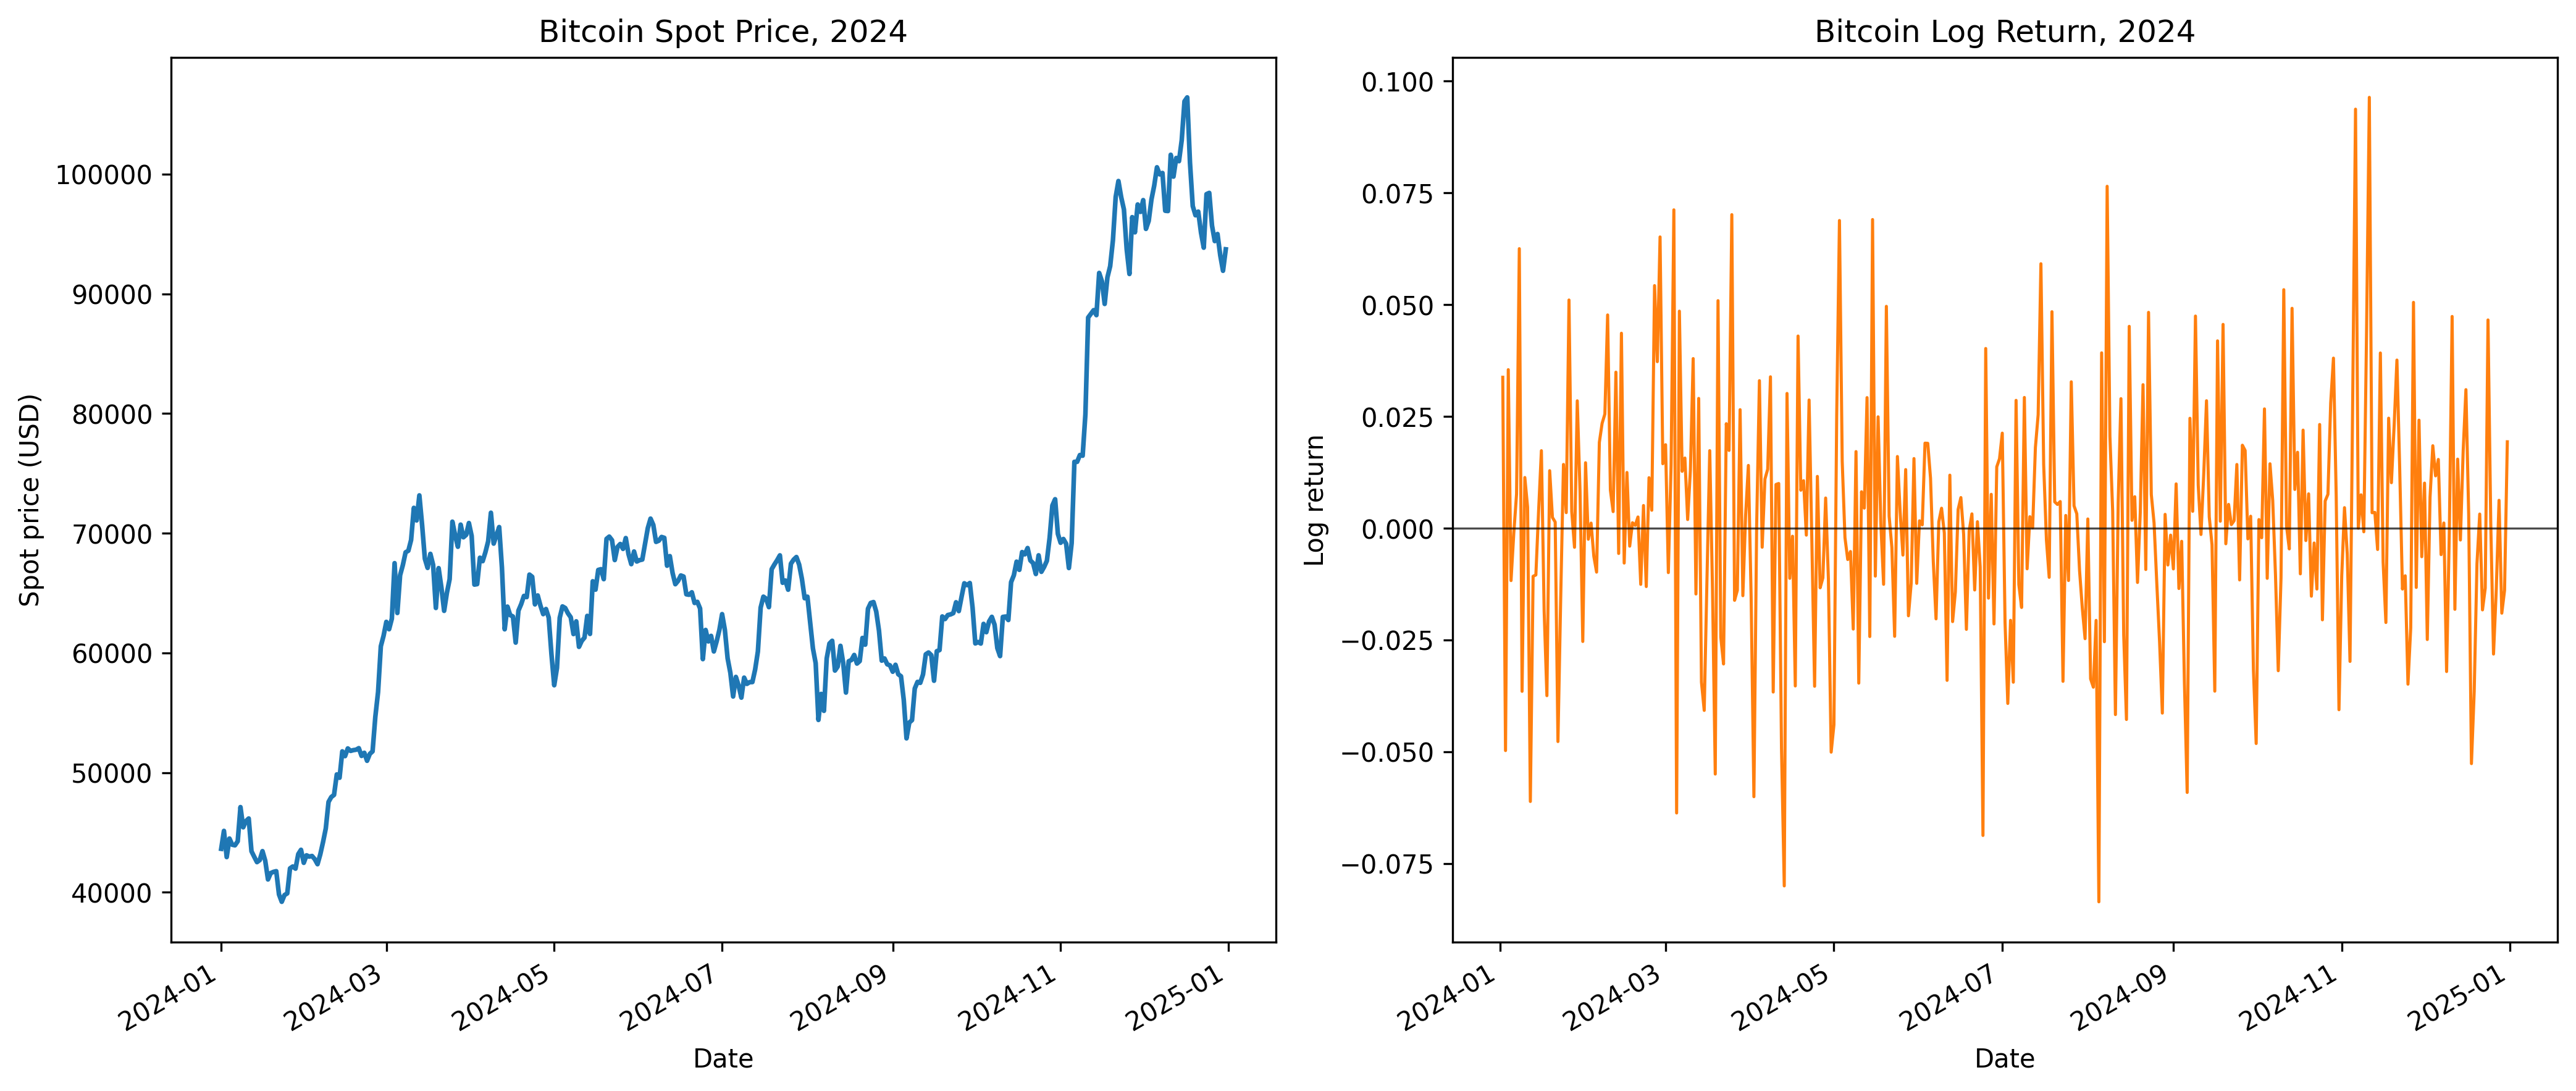
\includegraphics[width=\linewidth]{Sections/02_data_figures/btc_spot_and_log_return_2024.png}
    \caption{Bitcoin spot and log return time series for 2024}
    \label{fig:placeholder}
\end{figure}

The corresponding daily log return series (Figure 1, right panel) reveals the key distributional features that motivate the SVCJ modeling framework adopted in this thesis. As reported in Table 1, descriptive statistics for daily Bitcoin log returns over the full sample period from 2014 to 2024. The mean daily return of 0.001371 corresponds to an annualized return of approximately 50\%, yet the near-zero median of 0.000000 reveals that this long-run appreciation is driven by a small number of extraordinary return days rather than steady drift — a hallmark of a jump-driven process. The standard deviation of 0.034990 implies an annualized volatility of approximately 67\%, reflecting the repeated boom-and-bust cycles that characterize the decade, including the 2017–2018 crash, the March 2020 COVID collapse, and the 2021–2022 drawdown exceeding 70\%.

The distributional shape departs dramatically from normality along both dimensions of the Jarque-Bera decomposition. Skewness of -0.427 indicates a pronounced left tail: the largest single-day loss of -31.7\% substantially exceeds the largest single-day gain of +19.1\% in magnitude, reflecting crash episodes that pull the distribution asymmetrically downward and generate a downside jump risk premium embedded in Bitcoin option prices. Kurtosis of 9.754 — more than three times the Gaussian benchmark of 3 — confirms that extreme return realizations occur far more frequently than any normal distribution would predict. Jointly, these features produce a Jarque-Bera statistic of 7,527.47, constituting a categorical rejection of normality at any conventional significance level and closing the door on Black-Scholes as a viable pricing framework. These distributional facts collectively motivate the SVCJ specification adopted in this thesis, which explicitly accommodates stochastic volatility, correlated price jumps, and correlated volatility jumps as the minimum viable structure for capturing Bitcoin's return dynamics.

\begin{table}[h]
    \centering
    \begin{tabular}{cc}
    \hline
    \multicolumn{2}{c}{Descriptive statistics} \\
    \hline
        Mean & 0.001371 \\
        Standard deviation & 0.034990\\
        Skewness & $-0.426816$\\
        Kurtosis & 9.7541098\\
        Minimum & $-0.317282$\\
        Median & 0.000000\\
        Maximum & 0.190903\\
        JB & 7527.471506\\
        \hline
    \end{tabular}
    \caption{Descriptive statistics of Bitcoin log return (2014 to 2024)}
    \label{tab:placeholder}
\end{table}

\subsection{Deribit BTC Inverse Options and Daily Closing Prices}
\label{subsec:deribit_filtered_options}

The options dataset consists of intraday transaction records for European-style BTC inverse options traded on Deribit, the dominant venue for Bitcoin option trading. Inverse options are denominated and settled in Bitcoin rather than US dollars, so the BTC-denominated payoff differs from the payoff of a standard USD-settled option. This payoff convention is retained throughout the empirical analysis because the risk-neutral calibration is performed in the original BTC price units observed in the market.

Daily risk-neutral calibration requires a cross-section of option prices that refers, as closely as the data permit, to a common valuation time. Pooling all transactions over a 24-hour trading day would mix contracts traded under different intraday spot prices, volatility states, and remaining maturities. We therefore anchor each daily cross-section at 08:00 UTC, the natural Deribit settlement and option-expiration time. Because exact 08:00 transaction prices are generally unavailable, we construct a transaction-based closing panel from actual regular outright trades observed in a short interval centered on 08:00 UTC.


\begin{figure}[h]
    \centering
    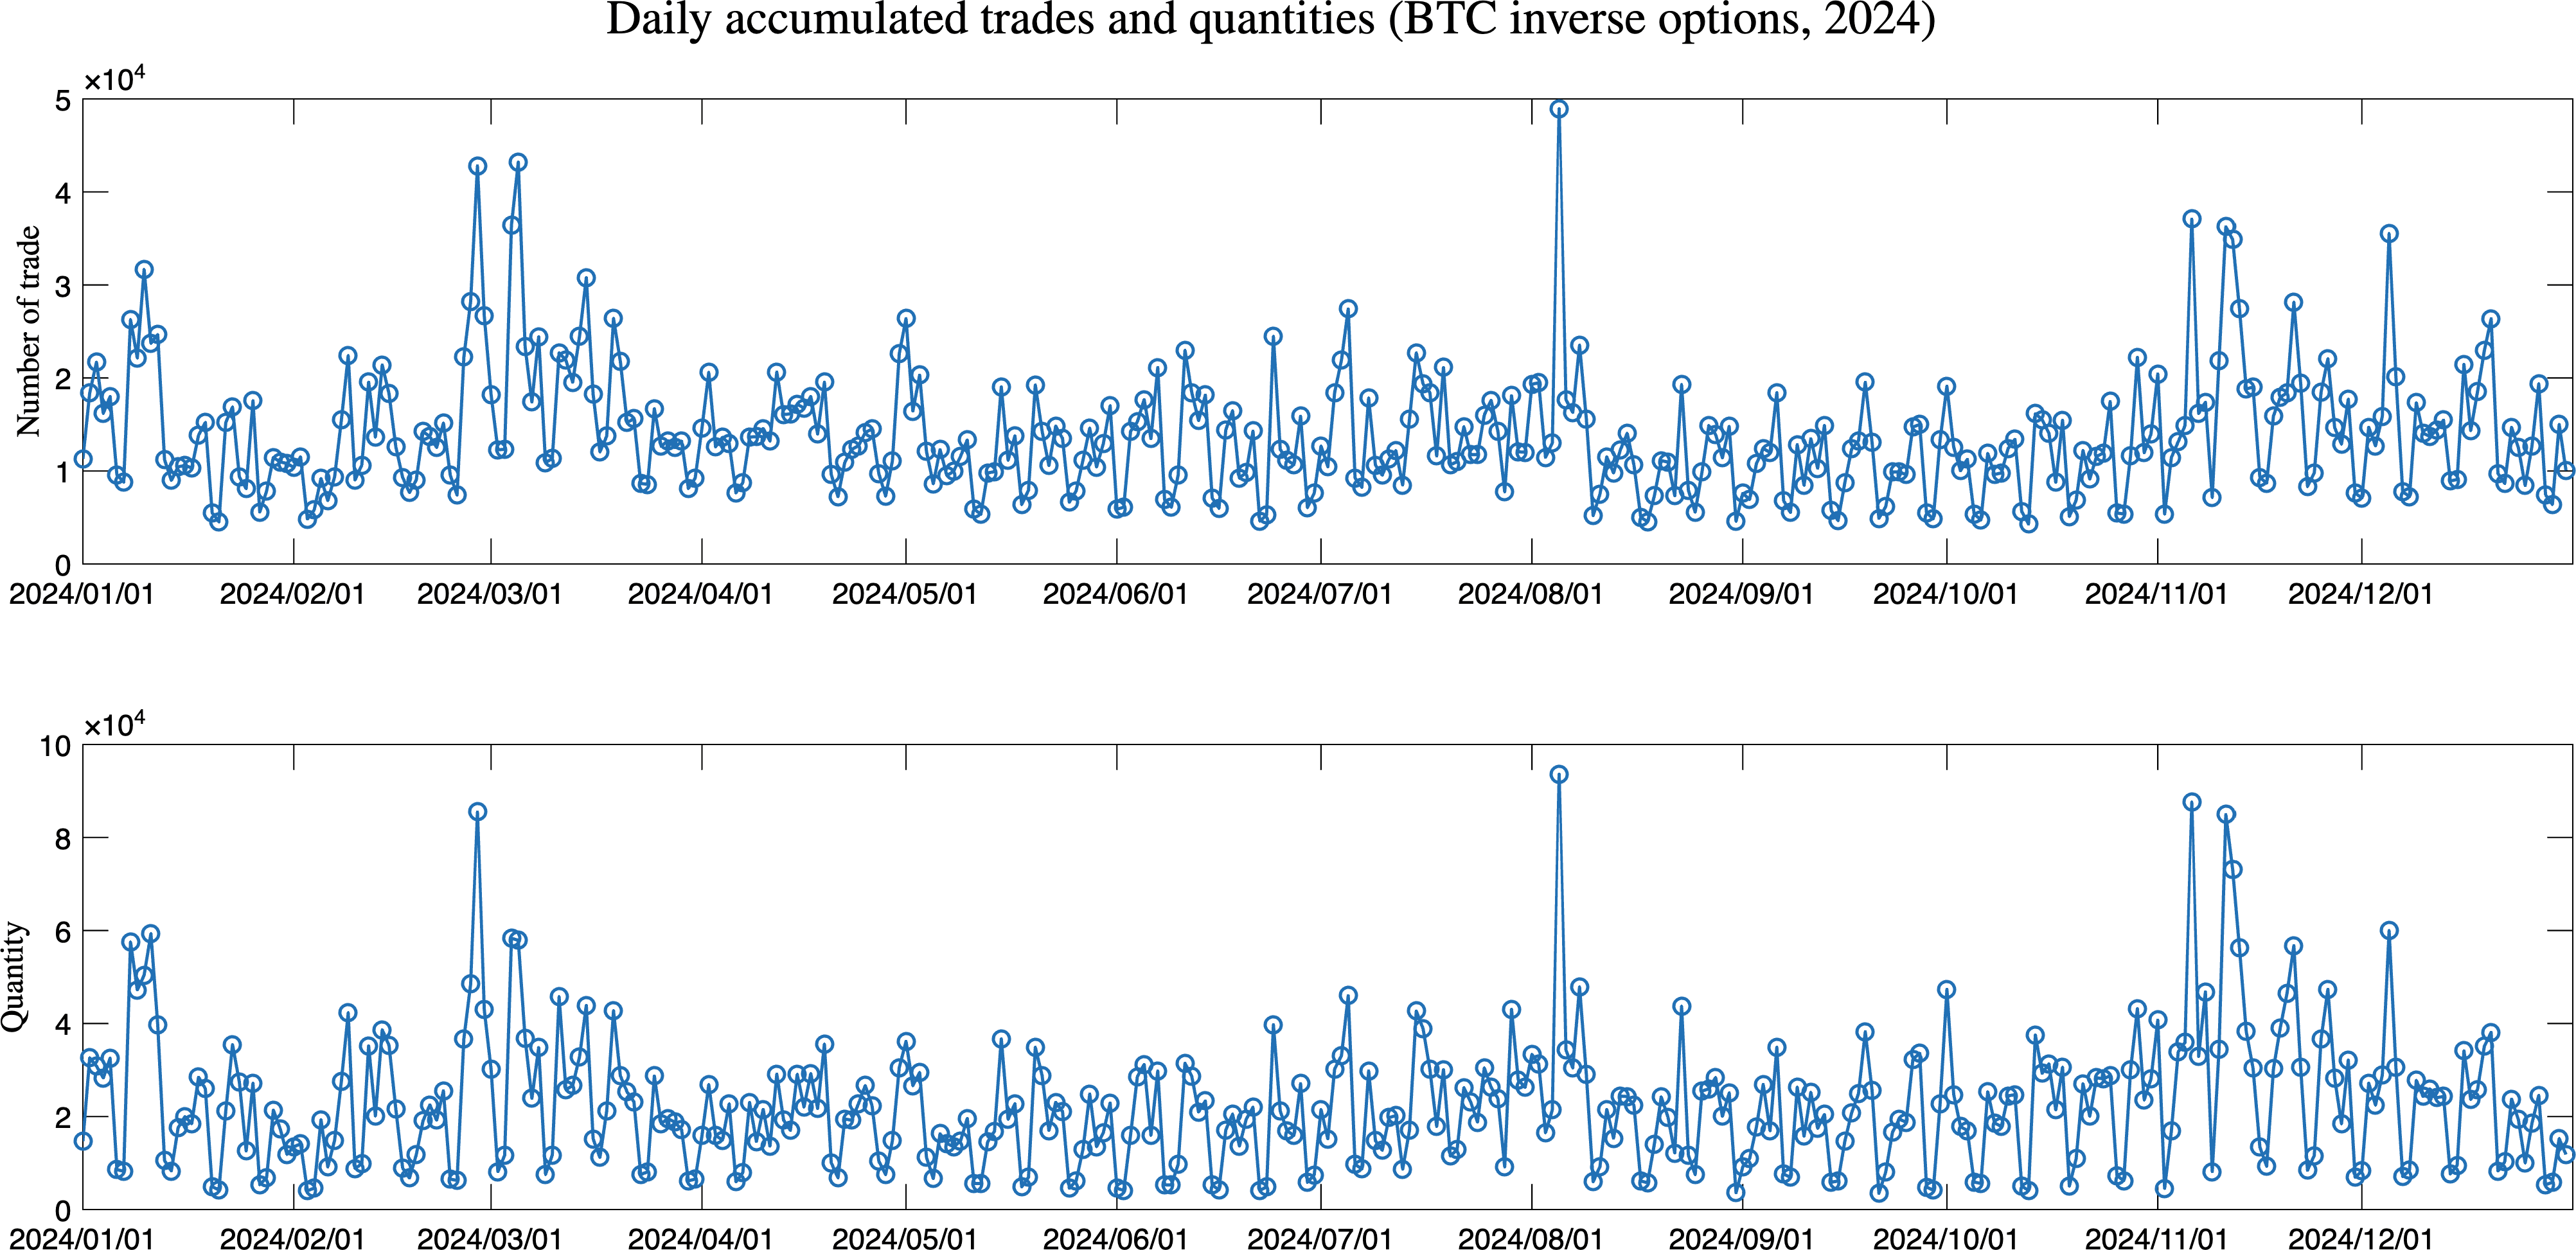
\includegraphics[width=\linewidth]{Sections/02_data_figures/Daily_traded_quantity.png}
    \caption{Daily accumulated trades and quantities}
    \label{fig:2024_daily_accu_trades_and_q}
\end{figure}

Figure~\ref{fig:2024_daily_accu_trades_and_q} shows daily trading activity throughout 2024, with the number of trades fluctuating between approximately 5,000 and 45,000 per day and total daily quantity ranging between 5,000 and 90,000 BTC notional. Two prominent spikes in both trades and quantity are visible around late February to early March and late July to early August 2024, coinciding with periods of elevated Bitcoin price volatility and heightened hedging demand. The overall level of activity confirms that the Deribit market is sufficiently liquid to support the daily cross-sectional calibration undertaken in this thesis.

\clearpage

\begin{figure}[h]
    \centering
    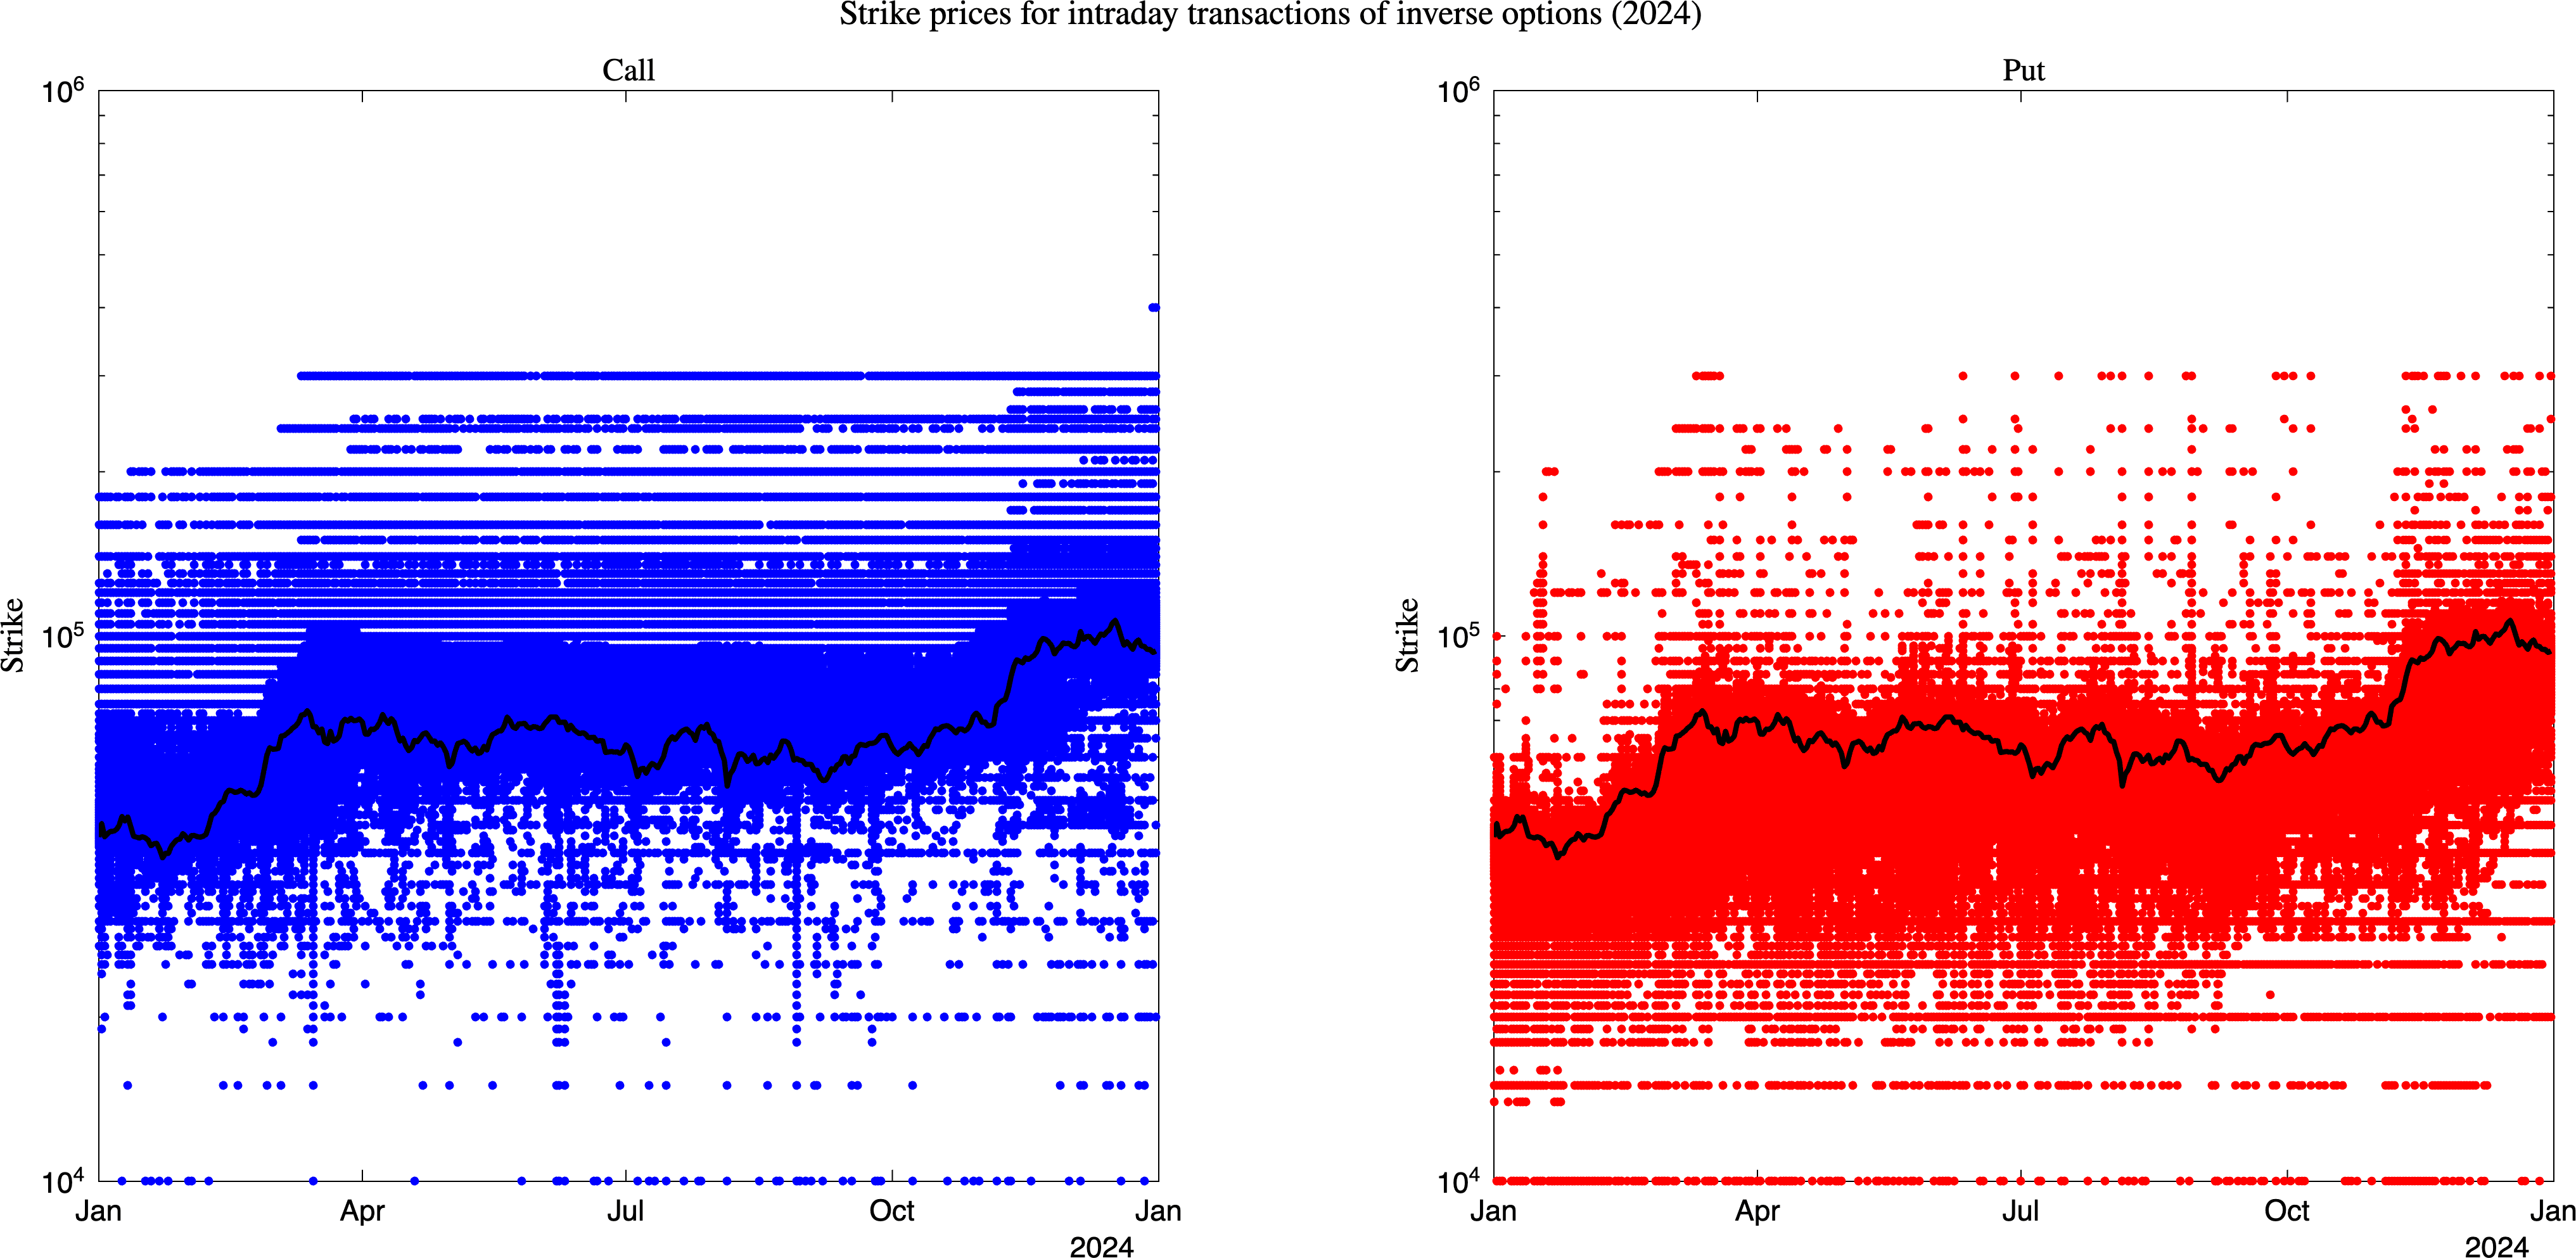
\includegraphics[width=\linewidth]{Sections/02_data_figures/Strike price for the intraday of inverse options.png}
    \caption{Visualizing strike prices for the intraday transaction of inverse
options}
    \label{fig:Prices_for_cp}
\end{figure}

Figure~\ref{fig:Prices_for_cp} illustrates the cross-sectional distribution of strike prices across the full year for calls (blue) and puts (red), with the black line tracing the daily spot price. Strikes span more than two orders of magnitude on a logarithmic scale – from approximately \$10,000 to \$1,000,000 – with the densest concentration in a band surrounding the at-the-money level, confirming that the most actively traded contracts are near-the-money options. The upward drift of the strike distribution mirrors the appreciation of the underlying spot price, indicating that market participants continuously recalibrate their hedging and speculative positions as BTC's price evolves.


For each UTC date and each instrument, let $\mathcal{I}_{j,d}(h)$ denote the set of eligible trades in the interval $[08{:}00-h,08{:}00+h]$, where $h$ is the half-window width. Liquidations, combination-strategy legs, block trades, and RFQ (Request for Quote) trades are excluded. The baseline closing price is the eligible trade closest to 08:00,
\begin{equation}
 p^{\mathrm{close}}_{j,d}
 =p_{i^{*},j,d}, \qquad
 i^{*}=\arg\min_{i\in\mathcal{I}_{j,d}(h)}
 \left|t_{i,j,d}-08{:}00\right|.
 \label{eq:closest_closing_trade}
\end{equation}
If multiple transactions are equally close, the larger transaction is selected, followed by the larger trade identifier as a deterministic tie-breaker. We also retain the quantity-weighted average price,
\begin{equation}
 p^{\mathrm{VWAP}}_{j,d}(h)
 =\frac{\sum_{i\in\mathcal{I}_{j,d}(h)}p_{i,j,d}q_{i,j,d}}
 {\sum_{i\in\mathcal{I}_{j,d}(h)}q_{i,j,d}},
 \label{eq:closing_vwap}
\end{equation}
and the median transaction price for robustness analysis. This panel is not an order-book snapshot: contracts without a qualifying transaction are not imputed.

Table~\ref{tab:closing_window_comparison_15min} compares 08:00-centered bandwidths from one to thirty minutes. Wider windows increase the number of available date--contract observations, but also move the selected trade farther from the target valuation time. The 15-minute half-window provides a practical compromise: it increases annual coverage from 27,018 observations under the five-minute window to 46,788 observations, and it captures a meaningfully broader set of longer-maturity contracts while retaining a tight 30-minute calendar window around the settlement time. We therefore use the 15-minute filtered panel as the experimental option dataset.

\begin{figure}[h]
    \centering
    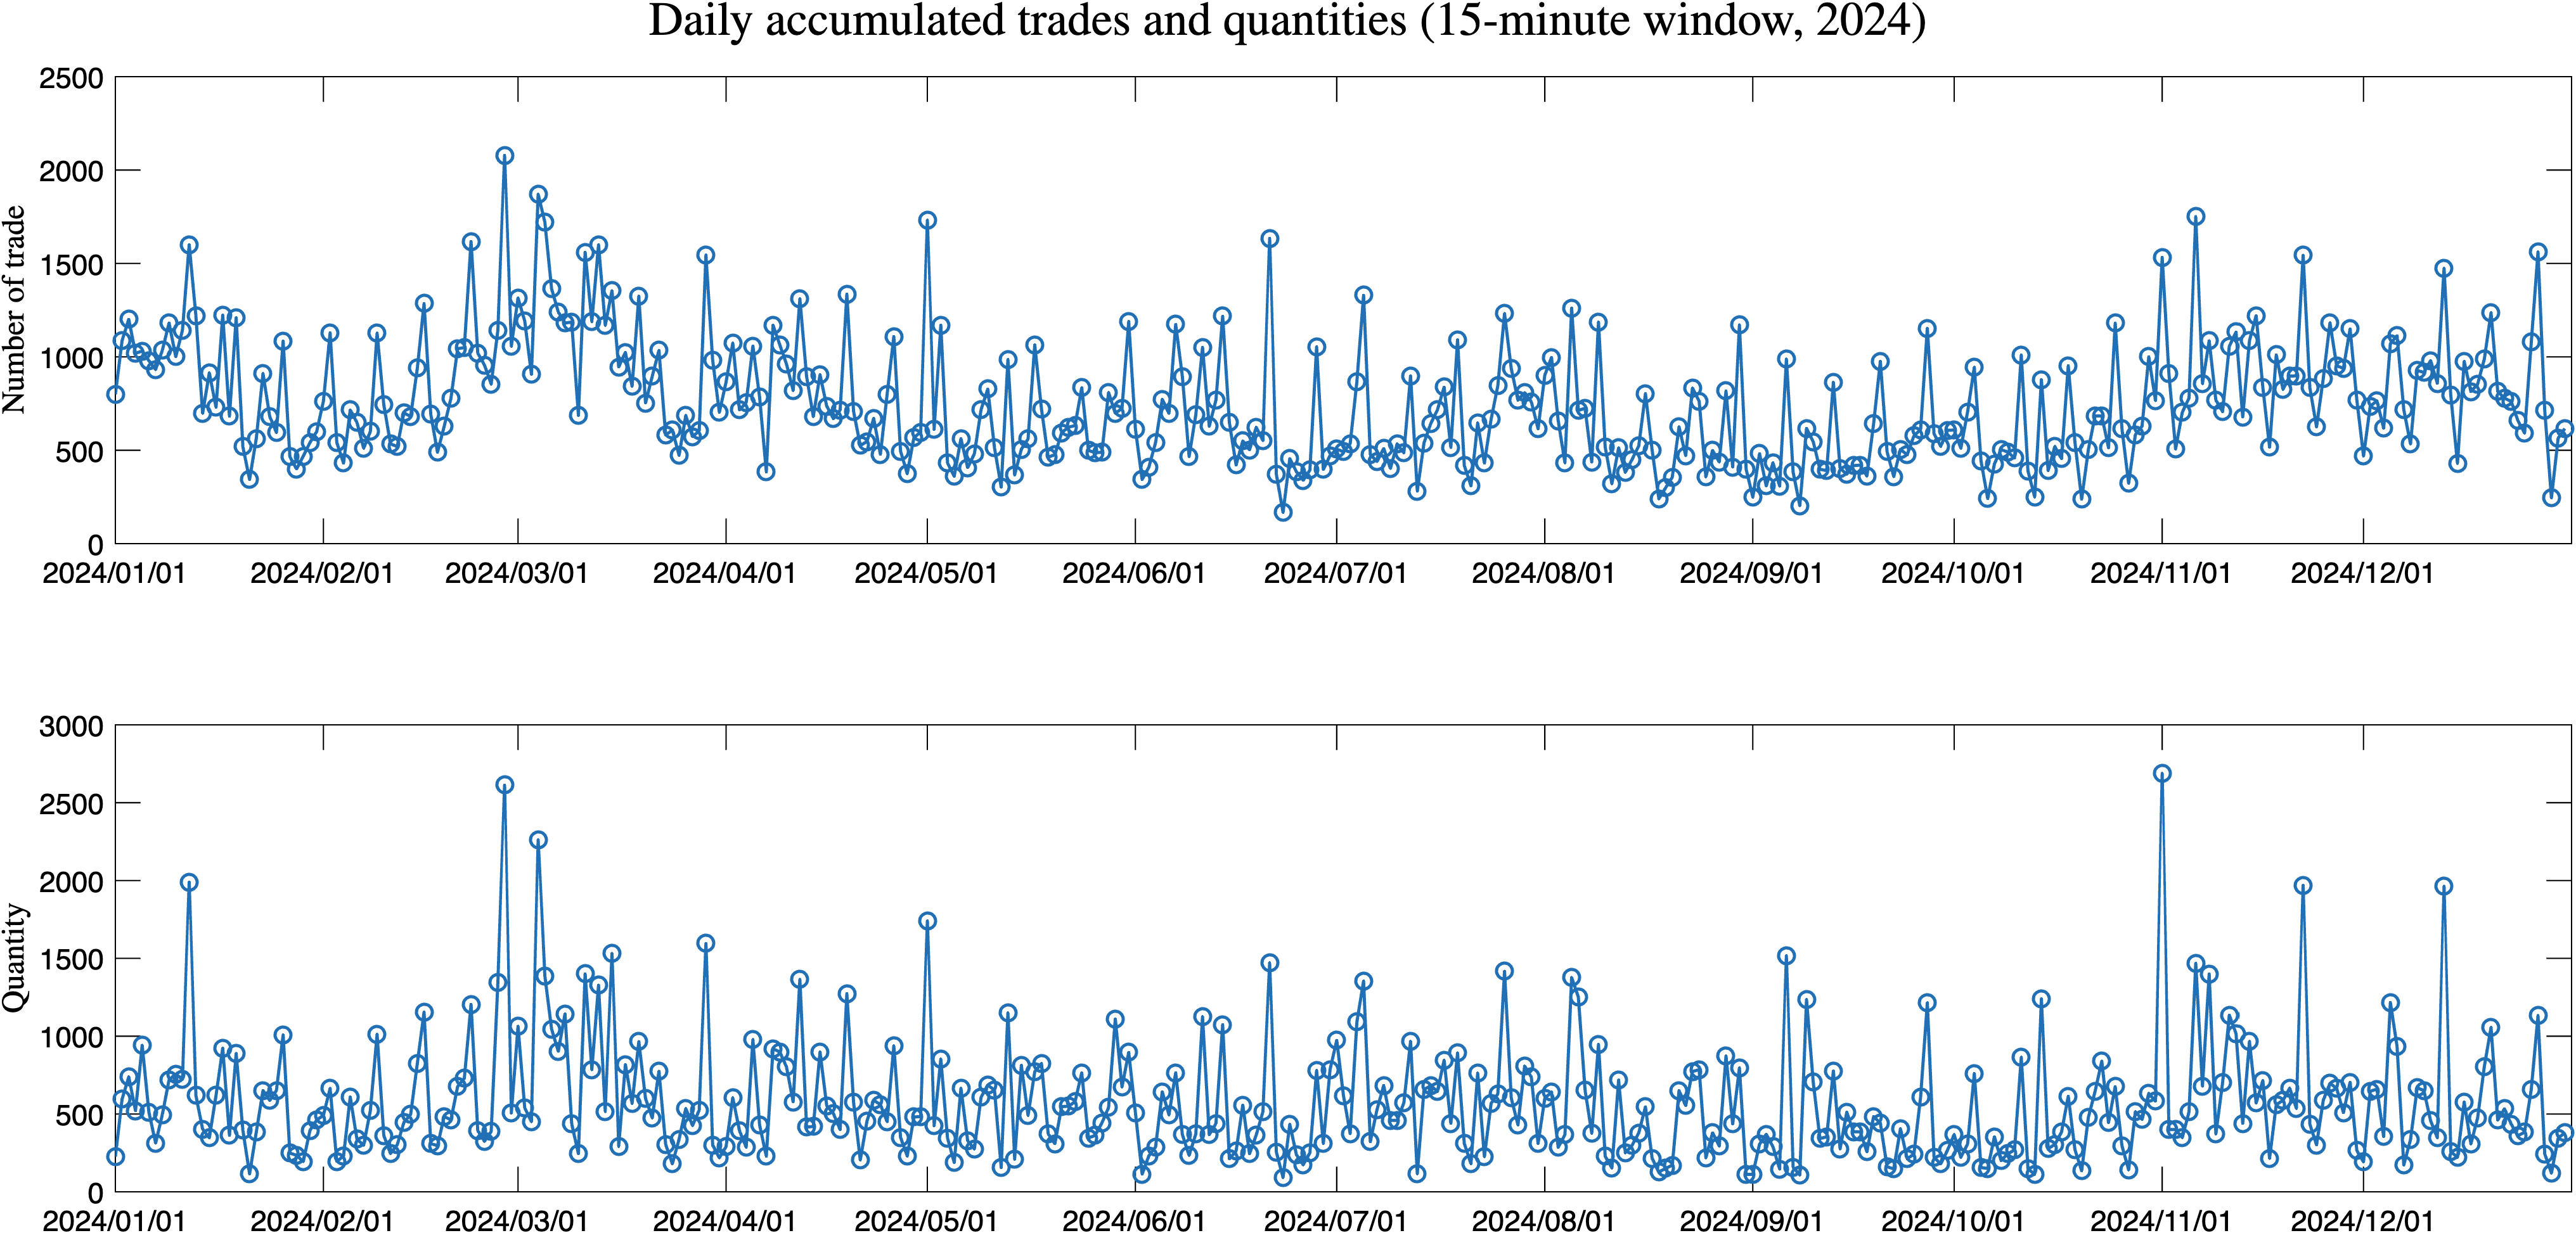
\includegraphics[width=\linewidth]{Sections/02_data_figures/Daily_traded_quantity_15min_filtered.png}
    \caption{Daily accumulated trades and quantities in the 15-minute filtered Deribit BTC inverse option panel}
    \label{fig:daily_quantity_15min_filtered}
\end{figure}

Figure~\ref{fig:daily_quantity_15min_filtered} shows trading activity inside the 15-minute closing window. The number of trades and total quantity vary substantially over time, with visible bursts around periods of elevated Bitcoin market activity. Since each retained date--contract observation is constructed from actual transactions near 08:00 UTC, the panel balances contemporaneous cross-sectional pricing with sufficient coverage for daily calibration.

\begin{figure}[h]
    \centering
    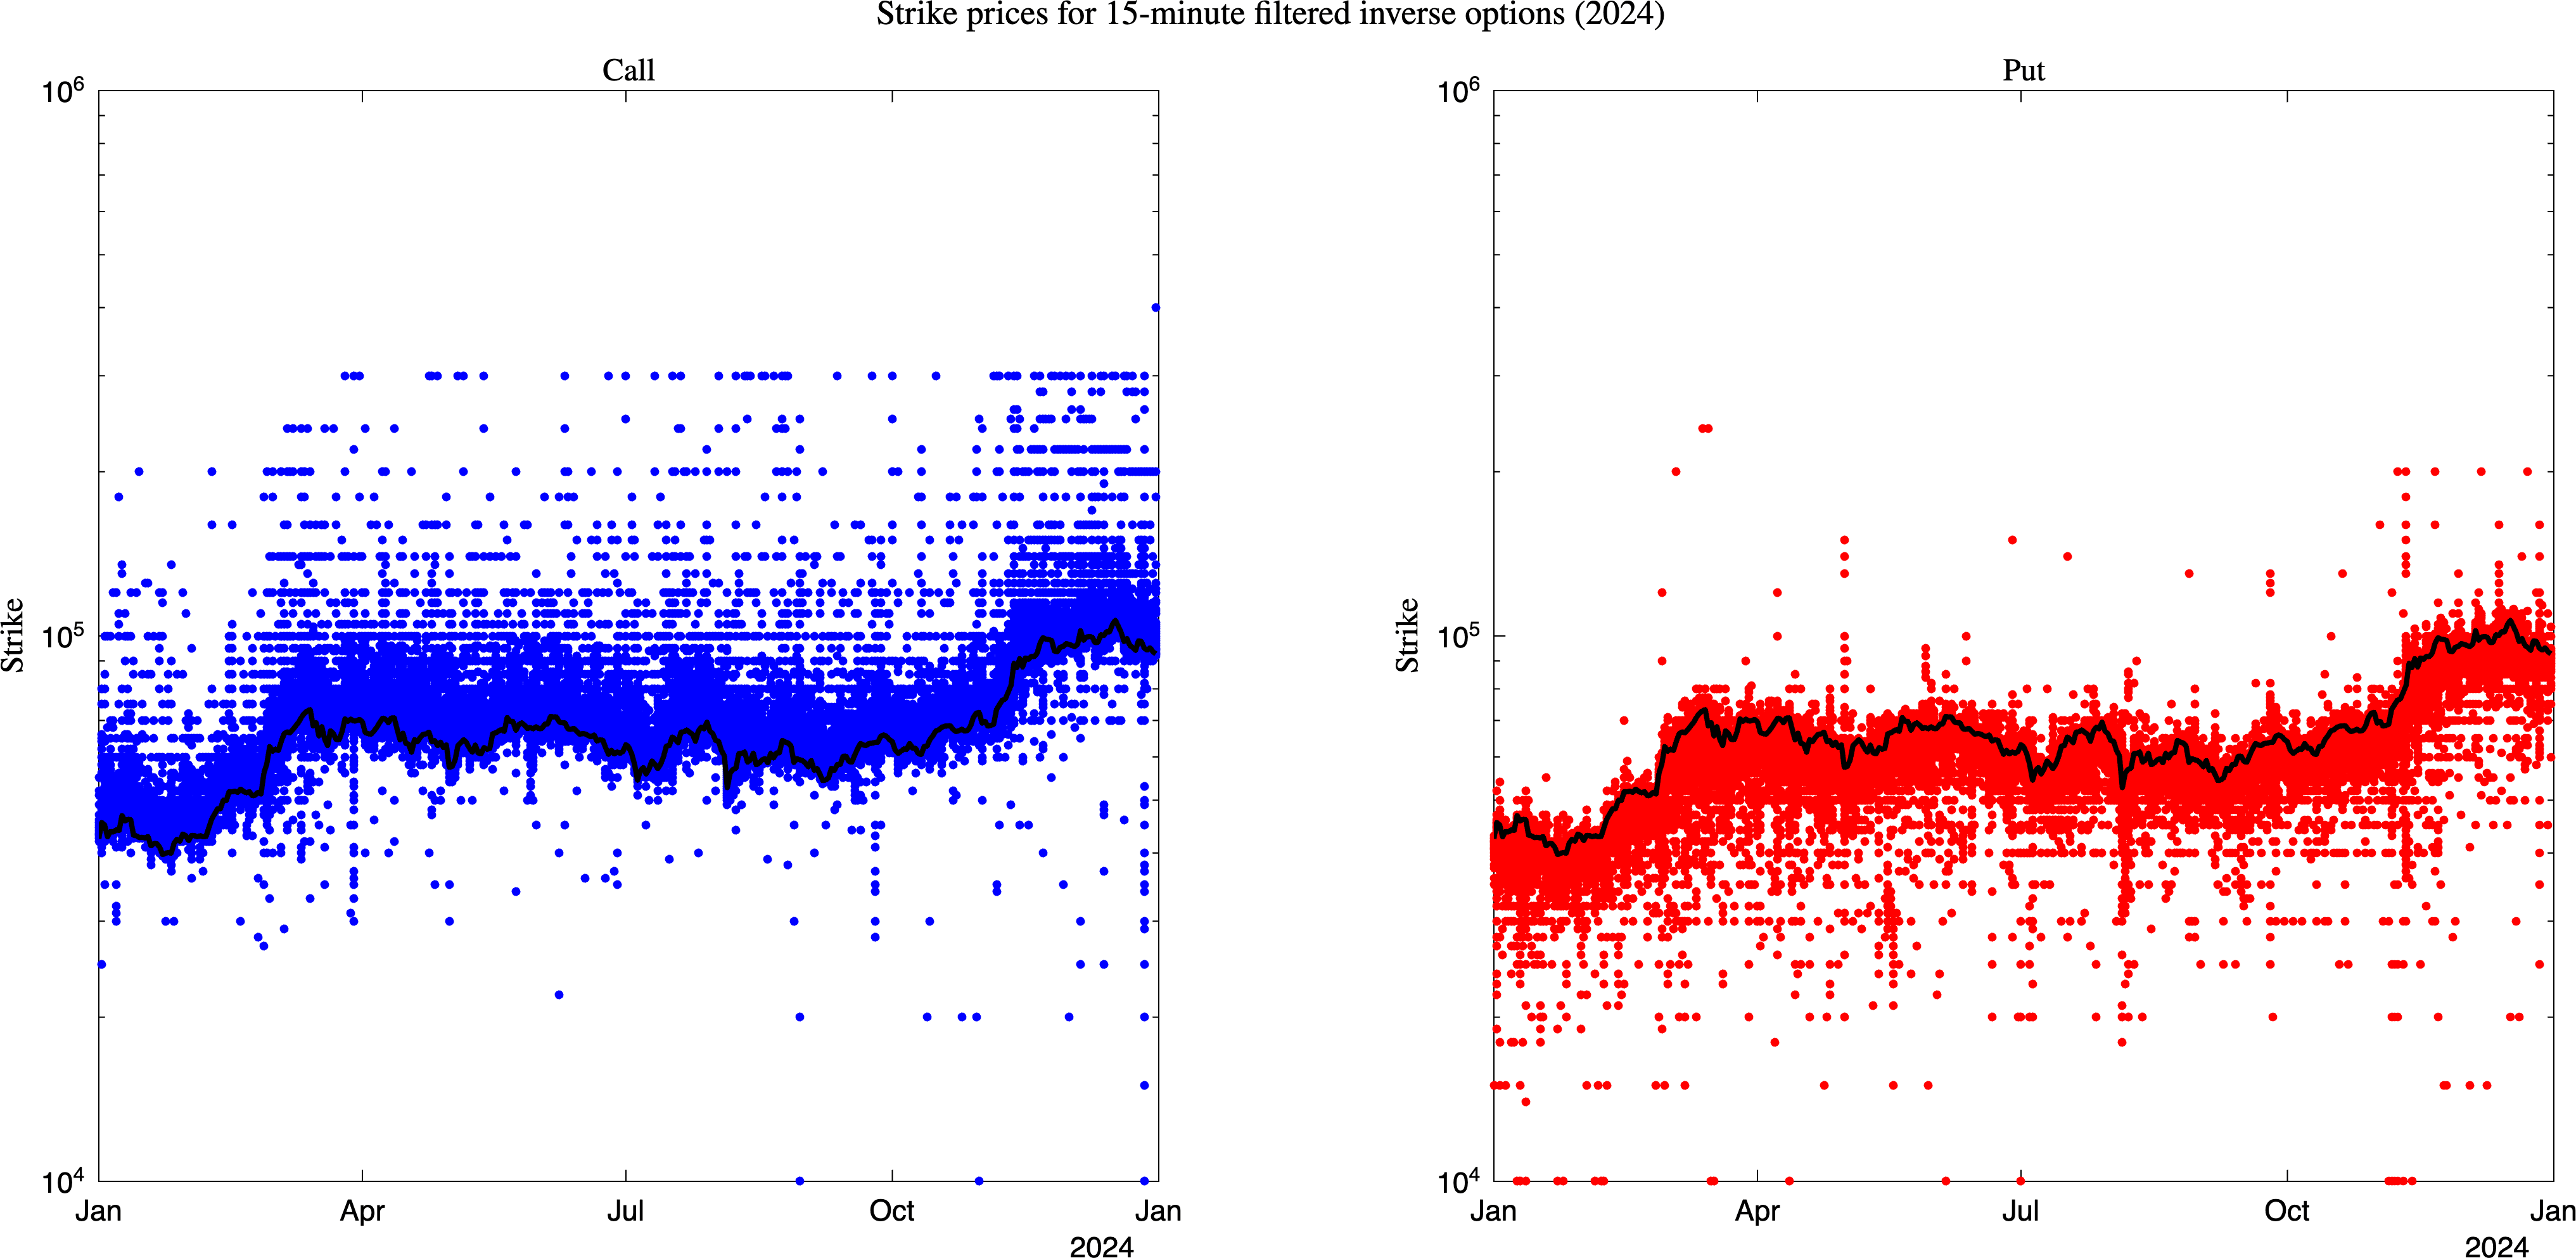
\includegraphics[width=\linewidth]{Sections/02_data_figures/Strike_price_15min_filtered_inverse_options.png}
    \caption{Visualizing strike prices for 15-minute filtered inverse BTC option observations}
    \label{fig:strike_15min_filtered}
\end{figure}

Figure~\ref{fig:strike_15min_filtered} displays the strike distribution of the filtered panel, with calls and puts shown separately and the 08:00 BTC index-price proxy overlaid in black. The filtered sample preserves a wide cross-section of strikes around the money while also retaining far out-of-the-money observations in both tails.

All maturity-related tables below use accurate time to maturity, measured from the selected transaction timestamp to the contract expiration timestamp. Thus an option traded exactly at 08:00 UTC one day before expiration has $T=1$, while a trade at 20:00 UTC one day before expiration would have $T=0.5$. In the 15-minute filtered panel this correction is small but conceptually important because the retained transaction need not occur exactly at 08:00.

\begin{table}[htbp]
\centering
\caption{\textbf{Comparison of daily closing-price windows.} For every UTC date in 2024, the table summarizes eligible regular outright BTC inverse-option transactions in a window centered on 08:00 UTC. Daily instruments counts distinct contracts with at least one eligible trade, and annual observations counts unique date--instrument pairs.}
\label{tab:closing_window_comparison_15min}
\begin{tabular}{lrrrrrr}
\toprule
Half-window & Full window & \multicolumn{2}{c}{Daily trades} & \multicolumn{2}{c}{Daily instruments} & Annual\\
\cmidrule(lr){3-4}\cmidrule(lr){5-6}
$h$ & width & Mean & Median & Mean & Median & observations\\
\midrule
$\pm 1$ min & 2 min & 52.76 & 45 & 22.27 & 21 & 8,151 \\
$\pm 2$ min & 4 min & 145.07 & 131 & 42.46 & 38 & 15,541 \\
$\pm 5$ min & 10 min & 411.99 & 366 & 73.82 & 66 & 27,018 \\
$\pm 10$ min & 20 min & 607.66 & 557 & 105.27 & 96 & 38,528 \\
$\pm 15$ min & 30 min & 756.87 & 698 & 127.84 & 118 & 46,788 \\
$\pm 20$ min & 40 min & 895.96 & 819 & 146.49 & 137 & 53,616 \\
$\pm 30$ min & 60 min & 1151.52 & 1034 & 176.33 & 166 & 64,537 \\
\bottomrule
\end{tabular}
\end{table}


\begin{table}[h]
\centering
\caption{\textbf{Distributions of 15-minute filtered option characteristics}. The table presents percentiles for BTC call and put options' accurate time to maturity ($T$), moneyness ($S_0/K$), and closest transaction prices ($p$).}
\label{tab:filtered_option_characteristics}
\begin{tabular}{lrrrrrr}
\hline
 & \multicolumn{2}{c}{T} & \multicolumn{2}{c}{S0/K} & \multicolumn{2}{c}{p} \\
 & Call & Put & Call & Put & Call & Put \\
\hline
Min & 0.00 & 0.00 & 0.19 & 0.29 & 0.0001 & 0.0001 \\
$Q_1$ & 0.00 & 0.00 & 0.40 & 0.87 & 0.0001 & 0.0001 \\
$Q_5$ & 1.00 & 1.00 & 0.65 & 0.96 & 0.0002 & 0.0002 \\
$Q_{10}$ & 1.00 & 1.00 & 0.75 & 0.98 & 0.0003 & 0.0003 \\
$Q_{20}$ & 1.01 & 1.00 & 0.85 & 1.00 & 0.0011 & 0.0010 \\
$Q_{30}$ & 2.00 & 2.00 & 0.89 & 1.02 & 0.0027 & 0.0021 \\
$Q_{40}$ & 3.00 & 2.01 & 0.92 & 1.03 & 0.0055 & 0.0041 \\
$Q_{50}$ & 7.00 & 4.99 & 0.94 & 1.05 & 0.0095 & 0.0075 \\
$Q_{60}$ & 12.00 & 8.99 & 0.96 & 1.08 & 0.0155 & 0.0120 \\
$Q_{70}$ & 18.01 & 14.01 & 0.98 & 1.10 & 0.0255 & 0.0195 \\
$Q_{80}$ & 35.00 & 25.00 & 0.99 & 1.15 & 0.0420 & 0.0325 \\
$Q_{90}$ & 72.00 & 56.99 & 1.01 & 1.27 & 0.0750 & 0.0580 \\
$Q_{95}$ & 122.99 & 88.99 & 1.05 & 1.44 & 0.1160 & 0.0895 \\
$Q_{99}$ & 291.51 & 254.00 & 1.26 & 2.16 & 0.2585 & 0.1835 \\
$Q_{99.9}$ & 356.99 & 351.72 & 2.41 & 4.46 & 0.6140 & 0.7303 \\
$Q_{99.99}$ & 364.00 & 362.00 & 6.14 & 7.60 & 0.8379 & 1.7365 \\
Max & 364.01 & 364.00 & 9.50 & 8.75 & 0.8960 & 2.1050 \\
\hline
\end{tabular}
\end{table}


Tables 2 and 3 report the same three characteristics - time to maturity ($T$), moneyness ($S_0/K$), and price ($p$) - but Table \ref{tab:weighted_option_characteristics} reweights each contract by traded volume rather than treating each observation equally. The comparison reveals a systematic shift in the bulk of the distribution once size is accounted for, while the extreme tails remain essentially unchanged.

For maturity, the weighted median maturity roughly doubles relative to the unweighted median (calls: 7 $\to$ 14 days; puts: 4 $\to$ 9 days), and this pattern persists through the 90th percentile (calls: 65 $\to$ 98; puts: 50 $\to$ 65). This indicates that larger trades are disproportionately concentrated in longer-dated contracts, rather than in the very short-dated options that dominate the raw contract count.

For moneyness, volume-weighting pulls the put-side distribution further out-of-the-money - the $Q_{90}$ for puts rises from 1.22 to 1.29 and $Q_{95}$
from 1.36 to 1.45 - while the call side is little changed or slightly more concentrated near-the-money at the median (0.96 $\to$ 0.93). This asymmetry is consistent with large-size trading activity being driven by downside/tail-hedging demand rather than symmetric directional speculation.

For price, reflecting both the longer maturities and deeper OTM put skew, weighted median prices are noticeably higher (calls: 0.0105 $\to$ 0.0162; puts: 0.0079 $\to$ 0.0105 BTC).

Notably, the extreme upper tail ($Q_{99.9}$ and beyond) is nearly identical across both tables for all three characteristics, since these percentiles are anchored by the same small set of extreme contracts regardless of weighting. The divergence is therefore a genuine feature of the bulk of the distribution, not an artifact of outliers - a useful diagnostic if you weight your Q-calibration loss function by trade size, since doing so will implicitly shift emphasis toward longer-dated, more OTM put contracts relative to an unweighted (per-contract) loss.


\begin{table}[h]
\centering
\caption{\textbf{Quantity-weighted distributions of 15-minute filtered option characteristics}. Percentiles are weighted by total contract quantity in each 15-minute window.}
\label{tab:filtered_weighted_option_characteristics}
\begin{tabular}{lrrrrrr}
\hline
 & \multicolumn{2}{c}{T} & \multicolumn{2}{c}{S0/K} & \multicolumn{2}{c}{p} \\
 & Call & Put & Call & Put & Call & Put \\
\hline
Min & 0.00 & 0.00 & 0.19 & 0.29 & 0.0001 & 0.0001 \\
$Q_1$ & 0.01 & 0.01 & 0.43 & 0.92 & 0.0001 & 0.0001 \\
$Q_5$ & 1.00 & 1.00 & 0.66 & 0.98 & 0.0002 & 0.0002 \\
$Q_{10}$ & 1.00 & 1.00 & 0.76 & 1.00 & 0.0004 & 0.0004 \\
$Q_{20}$ & 1.00 & 1.00 & 0.86 & 1.01 & 0.0013 & 0.0009 \\
$Q_{30}$ & 1.00 & 1.00 & 0.90 & 1.02 & 0.0029 & 0.0018 \\
$Q_{40}$ & 2.00 & 2.00 & 0.93 & 1.03 & 0.0050 & 0.0035 \\
$Q_{50}$ & 5.99 & 3.00 & 0.95 & 1.05 & 0.0080 & 0.0055 \\
$Q_{60}$ & 8.00 & 7.00 & 0.97 & 1.07 & 0.0120 & 0.0085 \\
$Q_{70}$ & 14.99 & 10.00 & 0.98 & 1.10 & 0.0180 & 0.0125 \\
$Q_{80}$ & 25.00 & 18.99 & 0.99 & 1.15 & 0.0300 & 0.0215 \\
$Q_{90}$ & 56.00 & 45.00 & 1.00 & 1.29 & 0.0525 & 0.0410 \\
$Q_{95}$ & 103.00 & 72.00 & 1.02 & 1.44 & 0.0810 & 0.0655 \\
$Q_{99}$ & 242.00 & 190.01 & 1.12 & 2.56 & 0.1785 & 0.1350 \\
$Q_{99.9}$ & 343.01 & 326.99 & 1.75 & 7.34 & 0.4595 & 0.2830 \\
$Q_{99.99}$ & 360.99 & 362.00 & 7.24 & 8.75 & 0.8645 & 0.6345 \\
Max & 364.01 & 364.00 & 9.50 & 8.75 & 0.8960 & 2.1050 \\
\hline
\end{tabular}
\caption{\textbf{Weighted distributions of option characteristics}. The table presents percentiles for BTC call and put options' time to maturity ($T$), moneyness ($S_0/K$), and prices ($p$), with $Q_k$ representing the $k$-th percentile.}
\label{tab:weighted_option_characteristics}
\end{table}


\begin{table}[h]
\centering
\caption{\textbf{Maturity-moneyness categories for 15-minute filtered options}. The table reports the proportion (\%) of date--contract observations in each category.}
\label{tab:filtered_maturity_moneyness_categories}
\begin{tabular}{lrrrr}
\hline
Inverse BTC call option & Deep OTM & OTM & ITM & \\
 & $\frac{S_0}{K} \leq 0.86$ & $0.86 < \frac{S_0}{K} \leq 1$ & $1 < \frac{S_0}{K}$ & Sum \\
\hline
Short-term: $T \leq 7$ & 1.5\% & 21.5\% & 4.2\% & 27.1\% \\
Mid-term: $7 < T \leq 28$ & 3.4\% & 8.0\% & 2.3\% & 13.7\% \\
Long-term: $28 < T$ & 6.7\% & 3.9\% & 1.4\% & 11.9\% \\
Sum & 11.5\% & 33.3\% & 7.9\% & 52.7\% \\
\hline
Inverse BTC put option & ITM & OTM & Deep OTM & \\
 & $\frac{S_0}{K} \leq 1$ & $1 < \frac{S_0}{K} \leq 1.12$ & $1.12 < \frac{S_0}{K}$ & Sum \\
\hline
Short-term: $T \leq 7$ & 4.5\% & 19.0\% & 3.4\% & 27.0\% \\
Mid-term: $7 < T \leq 28$ & 2.2\% & 5.3\% & 4.0\% & 11.4\% \\
Long-term: $28 < T$ & 1.7\% & 2.4\% & 4.9\% & 9.0\% \\
Sum & 8.3\% & 26.7\% & 12.3\% & 47.3\% \\
\hline
\end{tabular}
\end{table}

Tables \ref{tab:maturity_moneyness_categories} and \ref{tab:weighted_maturity_moneyness_categories} partition trading activity into a 3$\times$3 maturity-moneyness grid for calls and puts separately, contrasting the raw trade-count distribution (Table \ref{tab:maturity_moneyness_categories}) with the quantity-weighted distribution (Table \ref{tab:weighted_maturity_moneyness_categories}). Two consistent patterns emerge once volume is used as the weight instead of trade count.

Shift from short-term to long-term. Under the unweighted count, short-term options ($T\le 7$) dominate both calls (28.6\%) and puts (26.1\%), while long-term options are the smallest bucket (11.8\% calls, 7.7\% puts). Weighting by quantity essentially reverses this ordering for calls: long-term rises to 20.5\%, roughly matching short-term's 21.7\%, while for puts the short-term share nearly halves (26.1\% $\to$ 17.6\%) and long-term rises modestly (7.7\% $\to$ 9.7\%). This confirms what Table \ref{tab:weighted_option_characteristics} already suggested from the marginal maturity distribution — large trades cluster in longer-dated contracts, so a small number of big long-dated trades can rival a much larger number of small short-dated ones.

Shift toward deep OTM, especially at long maturities. The clearest movement is in the OTM/deep-OTM composition. For calls, deep-OTM share more than doubles for the long-term bucket alone (6.4\% $\to$ 12.4\%), and the overall call deep-OTM sum rises from 10.0\% to 17.1\%. For puts, the deep-OTM long-term cell rises from 4.2\% to 5.6\%, and overall put deep-OTM rises from 9.8\% to 11.8\%, while the near-the-money OTM bucket shrinks correspondingly (put OTM sum: 29.0\% → 22.6\%). This is consistent with the earlier percentile analysis: large trades skew toward tail hedges rather than near-the-money speculative flow.

Calls vs. puts asymmetry persists. Across both weighting schemes, calls retain a higher overall trading share than puts (55.1\% vs. 44.9\% unweighted; 60.6\% vs. 39.4\% weighted), and this gap widens under volume weighting — implying call-side activity is not just more frequent but carried out in larger size, plausibly reflecting basis-trade or covered-call-type flow that's naturally larger in inverse (BTC-margined) contracts.


\begin{table}[h]
\centering
\caption{\textbf{Quantity-weighted maturity-moneyness categories for 15-minute filtered options}. The table reports the proportion (\%) of total 15-minute window quantity in each category.}
\label{tab:filtered_weighted_maturity_moneyness_categories}
\begin{tabular}{lrrrr}
\hline
Inverse BTC call option & Deep OTM & OTM & ITM & \\
 & $\frac{S_0}{K} \leq 0.86$ & $0.86 < \frac{S_0}{K} \leq 1$ & $1 < \frac{S_0}{K}$ & Sum \\
\hline
Short-term: $T \leq 7$ & 1.6\% & 26.9\% & 3.3\% & 31.9\% \\
Mid-term: $7 < T \leq 28$ & 3.6\% & 8.8\% & 2.0\% & 14.5\% \\
Long-term: $28 < T$ & 6.6\% & 3.0\% & 0.7\% & 10.3\% \\
Sum & 11.8\% & 38.8\% & 6.1\% & 56.7\% \\
\hline
Inverse BTC put option & ITM & OTM & Deep OTM & \\
 & $\frac{S_0}{K} \leq 1$ & $1 < \frac{S_0}{K} \leq 1.12$ & $1.12 < \frac{S_0}{K}$ & Sum \\
\hline
Short-term: $T \leq 7$ & 3.2\% & 21.0\% & 3.5\% & 27.7\% \\
Mid-term: $7 < T \leq 28$ & 1.5\% & 4.2\% & 3.6\% & 9.3\% \\
Long-term: $28 < T$ & 0.9\% & 1.5\% & 3.9\% & 6.3\% \\
Sum & 5.6\% & 26.6\% & 11.1\% & 43.3\% \\
\hline
\end{tabular}
\caption{\textbf{Weighted Maturity-moneyness categories}. The table delineates nine categories based on maturity-moneyness. Short-term, mid-term, and long-term options are defined by $T \leq 7$, $7 < T \leq 28$, and $28 < T$, while OTM, ITM, and deep OTM options are defined by their moneyness ($S_0/K$). The table reports the proportion (\%) of trades in each maturity-moneyness category.}
\label{tab:weighted_maturity_moneyness_categories}
\end{table}

\begin{table}[h]
\centering
\caption{\textbf{Average prices in BTC and standard deviations for 15-minute filtered inverse options}. Standard deviations are in parentheses.}
\label{tab:filtered_average_prices_inverse_options}
\begin{tabular}{lccc}
\hline
Inverse BTC call option & Deep OTM & OTM & ITM \\
 & $\frac{S_0}{K} \leq 0.86$ & $0.86 < \frac{S_0}{K} \leq 1$ & $1 < \frac{S_0}{K}$ \\
\hline
Short-term: $T \leq 7$ & \makecell{0.0006\\(0.0008)} & \makecell{0.0045\\(0.0057)} & \makecell{0.0449\\(0.0694)} \\
Mid-term: $7 < T \leq 28$ & \makecell{0.0042\\(0.0045)} & \makecell{0.0228\\(0.0148)} & \makecell{0.0862\\(0.0742)} \\
Long-term: $28 < T$ & \makecell{0.0373\\(0.0422)} & \makecell{0.0794\\(0.0477)} & \makecell{0.2075\\(0.1449)} \\
\hline
Inverse BTC put option & ITM & OTM & Deep OTM \\
 & $\frac{S_0}{K} \leq 1$ & $1 < \frac{S_0}{K} \leq 1.12$ & $1.12 < \frac{S_0}{K}$ \\
\hline
Short-term: $T \leq 7$ & \makecell{0.0353\\(0.0551)} & \makecell{0.0045\\(0.0054)} & \makecell{0.0008\\(0.0012)} \\
Mid-term: $7 < T \leq 28$ & \makecell{0.0694\\(0.0554)} & \makecell{0.0219\\(0.0118)} & \makecell{0.0043\\(0.0040)} \\
Long-term: $28 < T$ & \makecell{0.1696\\(0.2020)} & \makecell{0.0617\\(0.0291)} & \makecell{0.0214\\(0.0225)} \\
\hline
\end{tabular}
\end{table}

\begin{table}[h]
\centering
\caption{\textbf{Quantity-weighted average prices in BTC and standard deviations for 15-minute filtered inverse options}. Weighted standard deviations are in parentheses.}
\label{tab:filtered_weighted_average_prices_inverse_options}
\begin{tabular}{lccc}
\hline
Inverse BTC call option & Deep OTM & OTM & ITM \\
 & $\frac{S_0}{K} \leq 0.86$ & $0.86 < \frac{S_0}{K} \leq 1$ & $1 < \frac{S_0}{K}$ \\
\hline
Short-term: $T \leq 7$ & \makecell{0.0005\\(0.0009)} & \makecell{0.0052\\(0.0060)} & \makecell{0.0303\\(0.0437)} \\
Mid-term: $7 < T \leq 28$ & \makecell{0.0058\\(0.0062)} & \makecell{0.0213\\(0.0142)} & \makecell{0.0778\\(0.0567)} \\
Long-term: $28 < T$ & \makecell{0.0334\\(0.0374)} & \makecell{0.0722\\(0.0446)} & \makecell{0.1976\\(0.1525)} \\
\hline
Inverse BTC put option & ITM & OTM & Deep OTM \\
 & $\frac{S_0}{K} \leq 1$ & $1 < \frac{S_0}{K} \leq 1.12$ & $1.12 < \frac{S_0}{K}$ \\
\hline
Short-term: $T \leq 7$ & \makecell{0.0275\\(0.0268)} & \makecell{0.0050\\(0.0053)} & \makecell{0.0008\\(0.0012)} \\
Mid-term: $7 < T \leq 28$ & \makecell{0.0645\\(0.0333)} & \makecell{0.0217\\(0.0123)} & \makecell{0.0037\\(0.0038)} \\
Long-term: $28 < T$ & \makecell{0.1347\\(0.1054)} & \makecell{0.0592\\(0.0304)} & \makecell{0.0172\\(0.0177)} \\
\hline
\end{tabular}
\caption{\textbf{Weighted average prices in BTC and standard deviations of inverse options.} This table displays the mean prices and standard deviations in parentheses for options across each maturity-moneyness category.}
\label{tab:weighted_average_prices_inverse_options}
\end{table}

Tables \ref{tab:average_prices_inverse_options} and \ref{tab:weighted_average_prices_inverse_options} report mean BTC-denominated prices (with standard deviations) across the same nine maturity-moneyness buckets, unweighted per-contract versus weighted by traded quantity. Three patterns stand out.

Monotonicity confirms internal consistency. Within both tables, prices rise monotonically with maturity for every moneyness bucket (as expected from time value), and rise monotonically with moneyness for calls (deep OTM cheapest, ITM most expensive) while falling monotonically with moneyness for puts. This is a useful sanity check: the data respects basic no-arbitrage ordering before any model fitting is applied, so any monotonicity violations you find later in the pricing kernel estimate can't be traced back to a raw data pathology at this level.

Weighting effects are asymmetric and bucket-specific, not uniform. Rather than a systematic upward or downward shift, quantity-weighting moves prices in different directions depending on the cell. Sh4ort-term ITM calls are notably more expensive when weighted (0.0326 → 0.0415), suggesting large trades in that bucket occurred disproportionately during high-price/high-vol windows. Conversely, long-term ITM puts are substantially cheaper when weighted (0.1761 → 0.1366) and long-term ITM calls slightly cheaper (0.1873 → 0.1787), suggesting the largest long-dated trades cluster in calmer pricing environments than the per-contract average implies. This bucket-dependent divergence means a single "volume-weighting effect" can't be assumed uniformly across your calibration grid — it needs to be checked cell by cell.

Dispersion is highest exactly where large trades concentrate. The standard deviations are large relative to the means in the long-term ITM buckets — long-term ITM puts show a standard deviation (0.2642 unweighted) that actually exceeds the mean (0.1761), a coefficient of variation above 1. Long-term deep-OTM calls show similar relative dispersion (0.0414 vs. mean 0.0374). Given that Tables 4–5 showed these same long-term/deep buckets are exactly where quantity-weighting shifts trading share upward, this dispersion is plausibly driven by the discrete macro-jump episodes (March, August, November) identified earlier — large trades executed in these buckets during the year likely span both pre- and post-jump price regimes, inflating within-bucket variance.

\clearpage

\subsection{Construction of Daily Closing Option Prices}
\label{subsec:daily_closing_prices}

Daily risk-neutral calibration requires a cross-section of option prices that refers, as closely as the data permit, to a common valuation time. If all transactions over a 24-hour period were pooled into one daily cross-section, differences across strikes and maturities would be confounded by intraday changes in the Bitcoin index, the implied-volatility state, and time to maturity. The resulting collection of prices would therefore not represent the option surface prevailing at any particular instant. This timing consideration is important for option-implied risk-neutral estimation, which treats prices across strikes as a contemporaneous cross-section \citep{AitSahaliaLo1998}. Recent empirical work on Bitcoin risk premia likewise illustrates the use of transaction-level option records organized at a daily frequency \citep{AlmeidaGrithMiftachovWang2024}.

We anchor the daily cross-section at 08:00 UTC. This is the natural boundary of a Deribit trading day: Deribit performs its daily settlement at 08:00 UTC, and its inverse BTC options expire at that time \citep{DeribitSettlement2026}. Exact 08:00 transaction prices are generally unavailable because an option contract need not trade at that instant. We consequently construct a daily closing transaction panel from actual outright trades observed in a short interval centered on 08:00 UTC. This panel should not be interpreted as a synchronous order-book snapshot: contracts without a qualifying transaction are not imputed, and historical bid and ask quotations are not used.

For each UTC date and each instrument, let $\mathcal{I}_{j,d}(h)$ denote the set of eligible trades in the interval $[08{:}00-h,08{:}00+h]$, where $h$ is the half-window width. Liquidations, combination-strategy legs, block trades, and RFQ (Request for quote) trades are excluded so that the retained observations represent regular outright market transactions. Our baseline closing price is the price of the eligible trade closest to 08:00,
\begin{equation}
 p^{\mathrm{close}}_{j,d}
 =p_{i^{*},j,d}, \qquad
 i^{*}=\arg\min_{i\in\mathcal{I}_{j,d}(h)}
 \left|t_{i,j,d}-08{:}00\right|.
 \label{eq:closest_closing_trade}
\end{equation}
If multiple transactions are equally close, the larger transaction is selected, followed by the larger trade identifier as a deterministic tie-breaker. To assess sensitivity to individual prints and bid--ask bounce, we also retain the quantity-weighted average price
\begin{equation}
 p^{\mathrm{VWAP}}_{j,d}(h)
 =\frac{\sum_{i\in\mathcal{I}_{j,d}(h)}p_{i,j,d}q_{i,j,d}}
 {\sum_{i\in\mathcal{I}_{j,d}(h)}q_{i,j,d}},
 \label{eq:closing_vwap}
\end{equation}
and the median transaction price for robustness analysis. Prices are preserved in their original BTC units. USD-equivalent prices are recorded separately by multiplying the BTC premium by the contemporaneous Deribit BTC index; this conversion changes the unit of account but does not transform an asynchronous trade into an exact 08:00 price.

Table~\ref{tab:closing_window_comparison} reports the coverage obtained from half-windows of one, two, and five minutes. The sample contains a qualifying transaction on every one of the 366 calendar days for all three specifications. A one-minute half-window produces only 22.27 distinct instruments per day on average, whereas a five-minute half-window increases average daily coverage to 73.82 instruments and yields 27,018 date--instrument observations over the year. The five-minute half-window, corresponding to 07:55--08:05 UTC, is therefore used to construct the preliminary closing panel. The closest-transaction price remains the baseline measure, while the five-minute VWAP and median price are retained for robustness checks. The shorter windows will be used to assess the sensitivity of the subsequent calibration to the trade-off between temporal synchronization and cross-sectional coverage.

\begin{table}[htbp]
\centering
\begin{tabular}{lrrrrrr}
\toprule
Half-window & Full window & \multicolumn{2}{c}{Daily trades} & \multicolumn{2}{c}{Daily instruments} & Annual\\
\cmidrule(lr){3-4}\cmidrule(lr){5-6}
$h$ & width & Mean & Median & Mean & Median & observations\\
\midrule
$\pm 1$ minute  & 2 minutes  & 52.76  & 45  & 22.27 & 21 & 8,151\\
$\pm 2$ minutes & 4 minutes  & 145.07 & 131 & 42.46 & 38 & 15,541\\
$\pm 5$ minutes & 10 minutes & 411.99 & 366 & 73.82 & 66 & 27,018\\
\bottomrule
\end{tabular}
\caption{\textbf{Comparison of daily closing-price windows.} For every UTC date in 2024, the table summarizes eligible regular outright BTC inverse-option transactions in a window centered on 08:00 UTC. ``Daily instruments'' counts distinct contracts with at least one eligible trade, and ``Annual observations'' counts unique date--instrument pairs. Liquidations, combination-strategy legs, block trades, and RFQ trades are excluded. All three windows contain at least one eligible transaction on each of the 366 sample days.}
\label{tab:closing_window_comparison}
\end{table}
\clearpage






\section{Preliminaries and our methodology}\label{sec:preliminaries}

\subsection{Physical-measure parameter estimation}
\label{subsec:p_parameter_estimation}

\subsubsection{SVCJ dynamics and MCMC estimation}
\label{subsubsec:p_svcj_mcmc}

We estimate the physical-measure SVCJ model from daily BTC/USD log returns.
The daily Euler transition is
\begin{align}
r_t &= \mu^P+\sqrt{V_{t-1}}\epsilon^y_t+J_t Z^y_t,
\label{eq:p_svcj_return}\\
V_t &= \alpha^P+\beta^P V_{t-1}
      +\sigma_v^P\sqrt{V_{t-1}}\epsilon^v_t+J_t Z^v_t,
\label{eq:p_svcj_variance}
\end{align}
where $\operatorname{corr}(\epsilon^y_t,\epsilon^v_t)=\rho^P$,
$J_t\sim\operatorname{Bernoulli}(\lambda^P)$,
$Z^v_t\sim\operatorname{Exp}(\mu_v^P)$, and
\begin{equation}
Z^y_t\mid Z^v_t
\sim\mathcal{N}\!\left(\mu_y^P+\rho_j^P Z^v_t,
                        (\sigma_y^P)^2\right).
\end{equation}
The exponential distribution is parameterized by its mean. The restrictions
$\alpha^P>0$ and $0<\beta^P<1$ imply the no-jump long-run variance
$\theta^P=\alpha^P/(1-\beta^P)$ and mean-reversion rate
$\kappa^P=1-\beta^P$.

We use Bayesian data augmentation to update the structural parameters jointly
with the latent variance path, jump indicators, and jump sizes. The first half
of every Markov chain is discarded as burn-in, and posterior means summarize
the retained draws. Successive rolling windows are warm-started from the
preceding posterior mean, while the latent jump indicators remain stochastic
states updated within the sampler rather than externally imposed observations.

\subsubsection{Simulation design for P-parameter recovery}
\label{subsubsec:p_parameter_recovery}

Before estimating the model from observed returns, we evaluate whether the
MCMC implementation can recover known physical-measure parameters and whether
recovery improves with sample length.  The data-generating vector follows the
reference implementation,
\begin{align}
\boldsymbol{\theta}^{P}_0
&=(\mu,\alpha,\beta,\sigma_v,\rho,\lambda,
   \mu_y,\sigma_y,\rho_j,\mu_v,V_0)' \\
&=(0.002,3.5\times10^{-5},0.95,0.005,-0.2,0.05,
   -0.01,0.11,-0.5,0.0006,0.0007)'.
\label{eq:p_simulation_true_parameters}
\end{align}
These values imply $\kappa=0.05$ and $\theta=0.0007$.  Estimation is carried
out in $(\alpha,\beta)$ because this is the sampler's natural parameterization;
the economically interpretable $(\kappa,\theta)$ are calculated from every
retained draw and reported alongside the directly sampled parameters.

We generate 20 independent master paths of 365 daily returns.  Within each
replication, estimation uses the nested prefixes
\begin{equation}
\mathcal{Y}_{30}\subset\mathcal{Y}_{90}
\subset\mathcal{Y}_{180}\subset\mathcal{Y}_{360},
\end{equation}
so changes across $n$ are not confounded by different simulated histories.
For every replication--sample-size pair, four chains start from deliberately
dispersed parameter vectors.  Each chain contains 100,000 MCMC sweeps, of
which the first 50,000 are discarded.  The sampler uses ancillary--sufficiency
interweaving between centered and noncentered variance representations and an
adaptive Fisher-transformed proposal for $\rho$ during burn-in.  Posterior
means and 90\% equal-tail credible intervals are computed from the pooled
retained draws of the four chains.

For parameter $j$ and replication $b$, absolute percentage error is
\begin{equation}
\operatorname{APE}_{jb}(n)
=100\left|\frac{\widehat\theta_{jb}(n)-\theta_{0,j}}
{\theta_{0,j}}\right|.
\label{eq:p_parameter_ape}
\end{equation}
The reported mean APE averages this quantity across the 20 replications.
We additionally calculate across-replication bias, RMSE, and empirical coverage
of the 90\% credible interval.  Mixing is evaluated separately for each
replication--sample-size pair using rank-normalized split $\widehat R$, bulk
effective sample size (ESS), and tail ESS.  A group passes only if every
reported parameter and the stored conditional log-likelihood statistic satisfy
$\widehat R\leq1.01$, bulk ESS $\geq400$, tail ESS $\geq400$, and contain no
nonfinite draws.  Estimates from failed groups remain in the table rather than
being selectively discarded.

\begin{table}[htbp]
\centering
\scriptsize
\resizebox{\textwidth}{!}{%
\begin{tabular}{lrrrrrrrrr}
\toprule
& & \multicolumn{2}{c}{$n=30$} & \multicolumn{2}{c}{$n=90$}
& \multicolumn{2}{c}{$n=180$} & \multicolumn{2}{c}{$n=360$}\\
\cmidrule(lr){3-4}\cmidrule(lr){5-6}\cmidrule(lr){7-8}\cmidrule(lr){9-10}
Parameter & True value & Estimate & APE (\%) & Estimate & APE (\%)
& Estimate & APE (\%) & Estimate & APE (\%)\\
\midrule
$V_0$      & 0.000700 & 0.001716 & 145.2 & 0.001745 & 149.2 & 0.001733 & 147.6 & 0.001594 & 127.8\\
$\mu$      & 0.002000 & 0.001409 & 184.8 & 0.002376 & 140.0 & 0.001358 & 87.3 & 0.001865 & 64.4\\
$\mu_y$    & $-0.010000$ & $-0.030602$ & 443.0 & $-0.006171$ & 480.1 & 0.001230 & 577.9 & 0.010539 & 514.4\\
$\sigma_y$ & 0.110000 & 0.115416 & 7.7 & 0.102549 & 12.9 & 0.095541 & 21.0 & 0.100355 & 21.7\\
$\lambda$  & 0.050000 & 0.050223 & 20.3 & 0.049696 & 32.4 & 0.052934 & 33.8 & 0.047834 & 33.2\\
$\alpha$   & 0.000035 & 0.001018 & 2809.5 & 0.000697 & 1891.9 & 0.000557 & 1491.9 & 0.000231 & 560.5\\
$\beta$    & 0.950000 & 0.140858 & 85.2 & 0.294739 & 69.0 & 0.492150 & 48.2 & 0.774528 & 18.5\\
$\rho$     & $-0.200000$ & 0.022395 & 140.6 & 0.014006 & 133.5 & $-0.135420$ & 116.7 & $-0.175243$ & 88.0\\
$\sigma_v$ & 0.005000 & 0.010086 & 101.7 & 0.008700 & 74.0 & 0.008536 & 70.7 & 0.007985 & 59.7\\
$\rho_j$   & $-0.500000$ & $-0.129865$ & 98.5 & $-0.230553$ & 116.2 & $-0.253463$ & 174.7 & 0.120796 & 208.3\\
$\mu_v$    & 0.000600 & 0.008831 & 1371.8 & 0.005503 & 817.2 & 0.002990 & 398.4 & 0.002004 & 233.9\\
$\kappa$   & 0.050000 & 0.859142 & 1618.3 & 0.705261 & 1310.5 & 0.507850 & 915.7 & 0.225472 & 350.9\\
$\theta$   & 0.000700 & 0.001167 & 75.3 & 0.000960 & 46.4 & 0.001000 & 45.6 & 0.001026 & 47.8\\
\midrule
Convergence pass & & \multicolumn{2}{c}{13/20} & \multicolumn{2}{c}{0/20}
& \multicolumn{2}{c}{0/20} & \multicolumn{2}{c}{1/20}\\
\bottomrule
\end{tabular}%
}
\caption{\textbf{Simulation-based recovery of physical-measure SVCJ parameters.}
The table reports posterior means and mean absolute percentage errors across
20 independent replications.  Each replication uses nested return samples and
four chains with 50,000 retained draws per chain.  The final row reports the
number of replication--sample-size groups satisfying all $\widehat R$ and ESS
criteria.  APE is computed within each replication before averaging and is
therefore not generally equal to the percentage error of the reported mean.}
\label{tab:p_parameter_recovery_simulation}
\end{table}

Table~\ref{tab:p_parameter_recovery_simulation} shows that longer return
histories improve some parameters but do not establish successful joint
recovery.  Mean APE for $\kappa$ declines monotonically from 1,618.3\% at
$n=30$ to 350.9\% at $n=360$, while the directly estimated $\beta$ improves
from 85.2\% to 18.5\%.  Nevertheless, the mean estimate
$\widehat\kappa=0.2255$ at $n=360$ remains more than four times its true value.
The APE of $\theta$ falls from 75.3\% to 46.4\% between $n=30$ and $n=90$ but
does not improve thereafter.  The variance-jump mean $\mu_v$, return-jump mean
$\mu_y$, and co-jump loading $\rho_j$ also remain weakly recovered.

Convergence evidence is more restrictive than the APE pattern.  Thirteen of
20 groups pass all diagnostics at $n=30$, whereas none passes at $n=90$ or
$n=180$ and only one passes at $n=360$.  The higher pass rate for the shortest
sample should not be interpreted as superior identification: its posterior is
broad, so chains can overlap even while estimates remain inaccurate.  These
results indicate that ASIS and adaptive proposals alone do not resolve the
strong posterior dependence and weak finite-sample identification of the full
SVCJ parameter vector.  Accordingly, the exercise is evidence on the current
estimator's limitations rather than validation of rolling estimates.

\subsubsection{Estimation-window selection and QQ diagnostics}
\label{subsubsec:p_window_selection}

The estimation window must balance local adaptation against identification.
A short return window is insufficient for the joint SVCJ specification: it
contains eleven structural parameters and latent states, while the jump block
is informed by relatively few events.  The recovery experiment above shows
that even 360 observations do not reliably identify the full parameter vector.
This concern is consistent with the much longer daily samples used in the
literature. \citet{ErakerJohannesPolson2003}
estimate stochastic-volatility jump models from long S\&P~500 and Nasdaq
histories, and \citet{ChaimLaurini2018} use 1,840 daily Bitcoin observations.

We therefore adopt 1,000 returns as the baseline rolling window. For a market
that trades seven days per week, this corresponds to approximately 2.7 years
and contains about 50 jump days in expectation at the simulation value
$\lambda^P=0.05$.  This choice is a conservative response to the poor recovery
observed at $n\leq360$, not a claim that the present simulation has validated a
1,000-return window.  An expanding window and a 2,000-return window therefore
serve as robustness specifications, and all empirical estimates must be
accompanied by chain-level convergence diagnostics. For target date $t$, the
baseline window contains only returns dated strictly before $t$, which
prevents look-ahead bias.

Model adequacy is assessed with a QQ plot of the standardized diffusion
innovation after removing the posterior expected jump contribution,
\begin{equation}
\widehat\epsilon_t^y
=\frac{r_t-\widehat\mu^P
        -\widehat{J_tZ_t^y}}
       {\sqrt{\widehat V_{t-1}}}.
\label{eq:p_standardized_innovation}
\end{equation}
Under a correctly specified diffusion component, its central quantiles should
be close to those of a standard normal distribution. Tail deviations are
interpreted as residual misspecification, not as a requirement that raw
Bitcoin returns themselves be Gaussian.

\subsection{Risk-neutral parameter estimation}
\label{subsec:q_parameter_estimation}

\subsubsection{Risk-neutral SVCJ specification}
\label{subsec:q_svcj_specification}

We first validate the numerical recovery of the risk-neutral parameters before
applying the calibration procedure to observed option prices. This validation
is important because SVCJ calibration is a nonlinear inverse problem: several
combinations of stochastic-volatility and jump parameters can generate similar
option-price surfaces, Monte Carlo error perturbs the objective function, and a
local least-squares optimizer can converge to different solutions from
different initial values. A satisfactory fit to market prices alone therefore
does not establish that the implementation can recover the parameters that
generated those prices. The simulation study below supplies a controlled
environment in which the data-generating parameter vector is known.

Let $Y_t=\log S_t$. Under the risk-neutral measure $\mathbb{Q}$, the SVCJ
dynamics used in the simulation are
\begin{align}
dY_t
&=\left(r-\delta-\frac{1}{2}V_t-\lambda\kappa_J\right)dt
  +\sqrt{V_t}\,dW_t^S+J_t^Y\,dN_t,
\label{eq:q_svcj_log_price}\\
dV_t
&=\kappa(\theta-V_t)dt
  +\sigma_v\sqrt{V_t}\,dW_t^V+J_t^V\,dN_t,
\label{eq:q_svcj_variance}
\end{align}
where $dW_t^S dW_t^V=\rho\,dt$, $N_t$ is a Poisson process with
intensity $\lambda$, and the simultaneous variance and log-price jumps satisfy
\begin{align}
J_t^V&\sim\operatorname{Exp}(\mu_v),\\
J_t^Y\mid J_t^V&\sim
\mathcal{N}\!\left(\mu_y+\rho_JJ_t^V,\sigma_y^2\right).
\end{align}
Here $\operatorname{Exp}(\mu_v)$ is parameterized by its mean. The
risk-neutral compensator is
\begin{equation}
\kappa_J
=E^{\mathbb{Q}}\!\left[e^{J_t^Y}-1\right]
=\frac{\exp(\mu_y+\tfrac{1}{2}\sigma_y^2)}
       {1-\rho_J\mu_v}-1,
\label{eq:q_svcj_jump_compensator}
\end{equation}
which requires $1-\rho_J\mu_v>0$. This drift adjustment ensures that the
discounted underlying price is a martingale. The specification follows the
affine jump-diffusion framework of \citet{DuffiePanSingleton2000} and the SVCJ
model of \citet{ErakerJohannesPolson2003}.

All parameters and maturities in this diagnostic experiment are expressed in
daily units. With one Euler step per day, the implementation uses full
truncation, $V_k^+=\max(V_k,0)$, and updates
\begin{align}
Y_{k+1}
&=Y_k+\left(r-\delta-\frac{1}{2}V_k^+
            -\lambda\kappa_J\right)
  +\sqrt{V_k^+}\,Z_{k+1}^S+I_{k+1}J_{k+1}^Y,
\label{eq:q_svcj_euler_log_price}\\
V_{k+1}
&=\max\left\{0,
  V_k^++\kappa(\theta-V_k^+)
  +\sigma_v\sqrt{V_k^+}\,Z_{k+1}^V
  +I_{k+1}J_{k+1}^V\right\},
\label{eq:q_svcj_euler_variance}
\end{align}
where
\begin{equation}
Z_{k+1}^V=\rho Z_{k+1}^S
          +\sqrt{1-\rho^2}\,Z_{k+1}^{\perp},
\qquad
I_{k+1}=\mathbf{1}\{U_{k+1}<\lambda\}.
\end{equation}

\subsubsection{Simulation design for Q-parameter recovery}
\label{subsec:q_parameter_recovery_simulation}

The data-generating vector is
\begin{align}
\boldsymbol{\theta}^{\mathbb Q}_0
&=\left(V_0,\kappa,\theta,\sigma_v,\rho,\lambda, \mu_y,\sigma_y,\rho_J,\mu_v\right)^{T} \\ 
&=\left(0.0009,0.7425,0.0008,0.0489,-0.6245,
       0.0033,0.3166,0.1267,-1.0821,0.0206\right)^{T}.
\label{eq:q_simulation_true_parameters}
\end{align}
We set $S_0=40{,}000$ and $r=\delta=0$. The candidate contract grid
contains 52 distinct integer maturities spanning 1 to 365 days and 2,001
equally spaced log-moneyness values from $-0.50$ to $0.50$ at each maturity,
for a total of 104,052 distinct contracts. To avoid placing mechanically
large intrinsic-value observations in the loss, the grid retains an
out-of-the-money put when the strike is below the forward and an
at-the-money or out-of-the-money call otherwise. The contracts are shuffled
once using a fixed seed, and the samples are nested:
\begin{equation}
\mathcal D_{100}\subset\mathcal D_{1000}\subset\mathcal D_{10000}.
\end{equation}
Thus, $n$ denotes the number of distinct option prices used in calibration,
not the number of simulated paths.

For each of five replications, synthetic observed prices are formed from
20,000 paths simulated at $\boldsymbol{\theta}^{\mathbb Q}_0$. Contracts with
the same maturity share the same terminal-price sample, and the discounted
average vanilla payoff gives
\begin{equation}
P_i^{\mathrm{obs}}
=\frac{1}{M_D}\sum_{m=1}^{M_D}
 e^{-rT_i}\max\!\left\{\omega_i
 \left(S_{T_i}^{(m)}-K_i\right),0\right\},
\qquad M_D=20{,}000,
\label{eq:q_simulation_observed_price}
\end{equation}
where $\omega_i=1$ for a call and $\omega_i=-1$ for a put. The synthetic
validation uses standard USD vanilla payoffs so that the Monte Carlo pricing
and optimization pipeline can be isolated from the additional payoff
transformation required by Deribit inverse options. The inverse-payoff
implementation is validated separately before the market-data calibration.

The experiment uses independent common-random-number sets across the data and
estimation stages. Specifically,
\begin{equation}
P_i^{\mathrm{obs}}
=\widehat P_i(\boldsymbol{\theta}^{\mathbb Q}_0;Z^{D}),
\qquad
P_i^{\mathrm{model}}(\boldsymbol{\theta})
=\widehat P_i(\boldsymbol{\theta};Z^{E}),
\qquad Z^{D}\ne Z^{E},
\label{eq:q_independent_crn_design}
\end{equation}
with $M_E=20{,}000$ estimation paths. The estimation draws $Z^E$ are cached
and held fixed at every objective evaluation and for every start within a
replication. Hence the optimizer sees a deterministic objective, but the
true-parameter loss need not be zero because the data and estimation path sets
are independent. This design is more stringent than a same-CRN diagnostic,
under which the true parameter produces zero pricing error by construction.

\subsubsection{Calibration and recovery criterion}
\label{subsec:q_parameter_recovery_estimation}

For every replication and value of $n$, the ten parameters are estimated by
bounded nonlinear least squares using MATLAB's trust-region-reflective
\texttt{lsqnonlin} algorithm. The relative residual for contract $i$ is
\begin{equation}
r_i^{USD}(\boldsymbol{\theta})
=\frac{P_i^{\mathrm{obs, USD}}
       -P_i^{\mathrm{model, USD}}(\boldsymbol{\theta})}
       {\max\{P_i^{\mathrm{obs, USD}},10^{-4}S_0\}},
\label{eq:q_relative_residual_USD}
\end{equation}
or equivalently
\begin{equation}
r_i^{BTC}(\boldsymbol{\theta})
=\frac{P_i^{\mathrm{obs, BTC}}
       -P_i^{\mathrm{model, BTC}}(\boldsymbol{\theta})}
       {\max\{P_i^{\mathrm{obs, BTC}},10^{-4}\}},
\label{eq:q_relative_residual_BTC}
\end{equation}
and the estimator minimizes
\begin{equation}
\widehat{\boldsymbol{\theta}}_n^{\mathbb Q}
=\arg\min_{\boldsymbol{\theta}\in\Theta}
 \sum_{i\in\mathcal D_n}r_i(\boldsymbol{\theta})^2.
\label{eq:q_nonlinear_least_squares}
\end{equation}
The denominator prevents expensive near-the-money contracts from completely
dominating the tail options that help identify jump parameters. The parameter
bounds are
\begin{align*}
\boldsymbol{\ell}
&=(0.00005,0.05,0.00005,0.005,-0.999,
   0.00005,-0.50,0.005,-8.0,0.0005)^{\prime},\\
\boldsymbol{u}
&=(0.01000,2.00,0.01000,0.200,0.500,
   0.05000,0.80,0.500,2.0,0.1000)^{\prime}.
\end{align*}

These bounds are economically and numerically motivated regularization
restrictions rather than parameter ranges copied mechanically from a single
empirical study.  The support restrictions require
$V_0,\theta,\sigma_v,\lambda,\sigma_y,$ and $\mu_v$ to be positive, and
$\rho$ to lie strictly inside the correlation interval.  Because Bitcoin
trades continuously, the daily-variance bounds
$V_0,\theta\in[0.00005,0.01]$ correspond to annualized diffusive
volatilities of approximately 13.5\% to 191\% under a 365-day convention,
which accommodates both tranquil and stressed cryptocurrency regimes.  The
Brownian correlation range $\rho\in[-0.999,0.5]$ permits the empirically
important negative return--variance leverage channel while retaining moderate
positive dependence as a possibility.  The daily jump-probability range
$\lambda\in[0.00005,0.05]$ corresponds to approximately 0.018 to 18.25
expected jump days per year and prevents the jump component from becoming
either exactly absent or observationally indistinguishable from a high-frequency
diffusion.

The remaining jump-size bounds are deliberately broad.  The interval
$\mu_y\in[-0.5,0.8]$ permits large negative and positive conditional log-price
jumps, while $\sigma_y\in[0.005,0.5]$ permits substantial jump-size
dispersion.  The parameter $\rho_J\in[-8,2]$ is a loading of the variance jump
in the conditional mean of the return jump, not a correlation coefficient;
its negative region permits crashes to coincide with upward variance jumps.
Together with $\mu_v\in[0.0005,0.1]$, these bounds guarantee
$1-\rho_J\mu_v>0$ throughout the search region, so the risk-neutral jump
compensator in equation~\eqref{eq:q_svcj_jump_compensator} remains finite.

Finally, $\kappa\in[0.05,2]$ imposes positive variance mean reversion and is
adapted to the daily Euler implementation rather than taken directly from
continuous-time equity-index estimates.  In the shock-free Euler recursion,
the coefficient on lagged variance is $1-\kappa$; setting the upper bound to
two rules out coefficients with absolute value greater than one and therefore
excludes mechanically explosive mean-reversion dynamics.  The endpoint
$\kappa=2$ is retained as a numerical boundary but is not strictly
contractive.  We do not separately impose the diffusion Feller condition
$2\kappa\theta\geq\sigma_v^2$, because the data-generating calibration used
in the recovery experiment need not satisfy it and the implementation instead
enforces nonnegative simulated variance through full truncation.  Boundary-hit
frequencies are reported as an identification diagnostic; systematic contact
with a bound would motivate a dedicated sensitivity calibration rather than an
economic interpretation of the constrained estimate.

We use four deterministic mild-SV initial vectors. They begin from
economically regular stochastic-volatility regimes while holding the jump
parameters at the common neutral values
$(\lambda,\mu_y,\sigma_y,\rho_J,\mu_v)
=(0.003,0,0.05,0,0.02)$. This structured design proved more reliable than
widely dispersed random starts. Parameter scaling is start-dependent,
\begin{equation}
\mathrm{TypicalX}_j=\max\{|\theta_j^{(0)}|,10^{-3}\},
\end{equation}
and forward finite differences use a relative step of $10^{-2}$. The
true-parameter vector is not included among the starts. For each replication
we retain the solution with the smallest relative-residual sum of squares.

Parameter recovery is evaluated using absolute percentage error,
\begin{equation}
\operatorname{APE}_j
=100\left|
\frac{\widehat\theta_j-\theta_{0,j}}
     {\theta_{0,j}}
\right|.
\label{eq:q_parameter_ape}
\end{equation}
Table~\ref{tab:q_parameter_recovery_simulation} reports estimates averaged
across the five replications. APE is computed within each replication and
then averaged, so it is not generally equal to the percentage error of the
reported mean estimate.

\begin{table}[htbp]
\centering
\scriptsize
\resizebox{\textwidth}{!}{%
\begin{tabular}{lrrrrrrr}
\toprule
& & \multicolumn{3}{c}{Mean estimated parameter}
& \multicolumn{3}{c}{Mean APE (\%)}\\
\cmidrule(lr){3-5}\cmidrule(lr){6-8}
Parameter & True value & $n=100$ & $n=1{,}000$ & $n=10{,}000$
& $n=100$ & $n=1{,}000$ & $n=10{,}000$\\
\midrule
$V_0$      & 0.000900 & 0.001038 & 0.000933 & 0.000918 & 29.98 & 9.06  & 3.68\\
$\kappa$   & 0.742500 & 0.396534 & 0.561539 & 0.547842 & 46.59 & 24.37 & 26.22\\
$\theta$   & 0.000800 & 0.000856 & 0.000924 & 0.000897 & 15.13 & 21.49 & 14.86\\
$\sigma_v$ & 0.048900 & 0.038726 & 0.035032 & 0.038401 & 22.93 & 29.50 & 21.47\\
$\rho$     & $-0.624500$ & $-0.288091$ & $-0.667680$ & $-0.614877$ & 53.87 & 18.42 & 17.05\\
$\lambda$  & 0.003300 & 0.003844 & 0.003427 & 0.002961 & 16.63 & 25.50 & 21.96\\
$\mu_y$    & 0.316600 & 0.203652 & 0.318214 & 0.323335 & 35.68 & 23.14 & 14.92\\
$\sigma_y$ & 0.126700 & 0.044407 & 0.120930 & 0.120403 & 64.95 & 11.17 & 10.10\\
$\rho_J$   & $-1.082100$ & 1.848960 & $-0.145671$ & 1.054524 & 270.87 & 262.33 & 197.45\\
$\mu_v$    & 0.020600 & 0.018796 & 0.012498 & 0.009348 & 23.28 & 42.39 & 54.62\\
\midrule
Mean APE   & & & & & 57.99 & 46.74 & 38.23\\
Median APE & & & & & 32.83 & 23.75 & 19.26\\
\bottomrule
\end{tabular}%
}
\caption{\textbf{Simulation-based recovery of risk-neutral SVCJ parameters.}
The table reports results from five independent replications. Synthetic
observed prices and model prices use separate sets of 20,000 Monte Carlo paths.
For each replication, the calibration selects the lowest-loss solution among
four deterministic mild-SV starts. The option samples are nested across
$n=100$, $1{,}000$, and $10{,}000$. Mean APE is calculated parameter by
parameter across replications. The final two rows summarize the ten reported
parameter-specific APE values.}
\label{tab:q_parameter_recovery_simulation}
\end{table}

The cross-sectional increase in option count improves recovery on average.
The mean parameter APE decreases from 57.99\% at $n=100$ to 46.74\% at
$n=1{,}000$ and 38.23\% at $n=10{,}000$; the corresponding median falls from
32.83\% to 23.75\% and 19.26\%. Recovery improves especially for $V_0$,
$\rho$, $\mu_y$, and $\sigma_y$. The improvement is not uniform, however.
The co-jump parameter $\rho_J$ remains weakly identified, and the APE of
$\mu_v$ increases with $n$. These patterns are consistent with compensation
among jump intensity, jump-size, and co-jump parameters. They also show why
pricing fit alone cannot be treated as evidence of parameter identification.
Nevertheless, the decline in the central tendency of APE demonstrates that a
richer option cross-section provides useful recovery information, while the
remaining jump-parameter instability motivates the multiple-start,
diagnostic, and robustness procedures used in the market-data calibration.



\section{Empirical Analysis} \label{sec:empirical_analysis}

\subsection{Physical-measure estimates and diagnostics}
\label{sec:p-estimation-results}

For every calendar day in 2024, the information set contains the preceding
1,000 returns and excludes the return dated $t$, preventing look-ahead bias.
Each chain is warm-started from the preceding day's posterior mean and saved
immediately for restartability. The short-period diagnostic uses the final 90
returns of 2024. Its QQ plot is a specification diagnostic for the diffusion
innovation after removing posterior expected jumps; departures in the tails
therefore indicate residual misspecification rather than evidence that the raw
BTC return itself should be Gaussian.



\section{Conclusion} \label{sec:conclusion}


\singlespacing
\setlength\bibsep{0pt}
\bibliographystyle{chicago}
\bibliography{20260527_Chin_reference}

\clearpage


%\section*{Appendix A. Placeholder} \label{sec:appendixa}
%\addcontentsline{toc}{section}{Appendix A}
\section{Appendix}
\label{sec:appendix}
\begin{table}[h]
    \centering
    \begin{tabular}{llll}
         \hline
         Index & Column & Type & Description \\
         \hline
         1 & \textit{trade id} & string & Unique (per currency) trade identifier \\
         2 & $q$ & number & quantity \\
         3 & $p$ & number & Option price denoted in BTC \\
         4 & $d$ & string & Date (YYYY/mm/dd) \\
         5 & $iv$ & number & implied volatility \\
         6 & \textit{instrument name} & string & UNDERLYING-MATURITY-STRIKE (Call/Put) \\
         7 & \textit{direction} & string & buy/sell\\
         8 & \textit{index price} & number & underlying BTC index price denominated in USD \\
         \hline
         
    \end{tabular}
    \caption{\textbf{Fields in the original Deribit transaction dataset.} The table lists the variables retained from the Deribit API before construction of the closing-window panel.}
    \label{tab:appendix_deribit_transaction_fields}
\end{table}


\clearpage
\subsection{Full-Year Intraday Deribit BTC Inverse Option EDA}
\label{app:full_year_intraday_option_eda}

Table~\ref{tab:appendix_deribit_transaction_fields} describes the fields in the original transaction records. The full-year exploratory results below use all eligible 2024 intraday BTC inverse-option trades, rather than only the 15-minute closing-window observations used in Section~\ref{subsec:deribit_filtered_options}. Inverse options are denominated and settled in Bitcoin rather than US dollars; for example, the BTC-settled call payoff is $\max\{(S_T-K)/S_T,0\}$ BTC. Multiplying this payoff by $S_T$ recovers the usual USD payoff $\max\{S_T-K,0\}$.

% \clearpage

\begin{figure}[h]
    \centering
    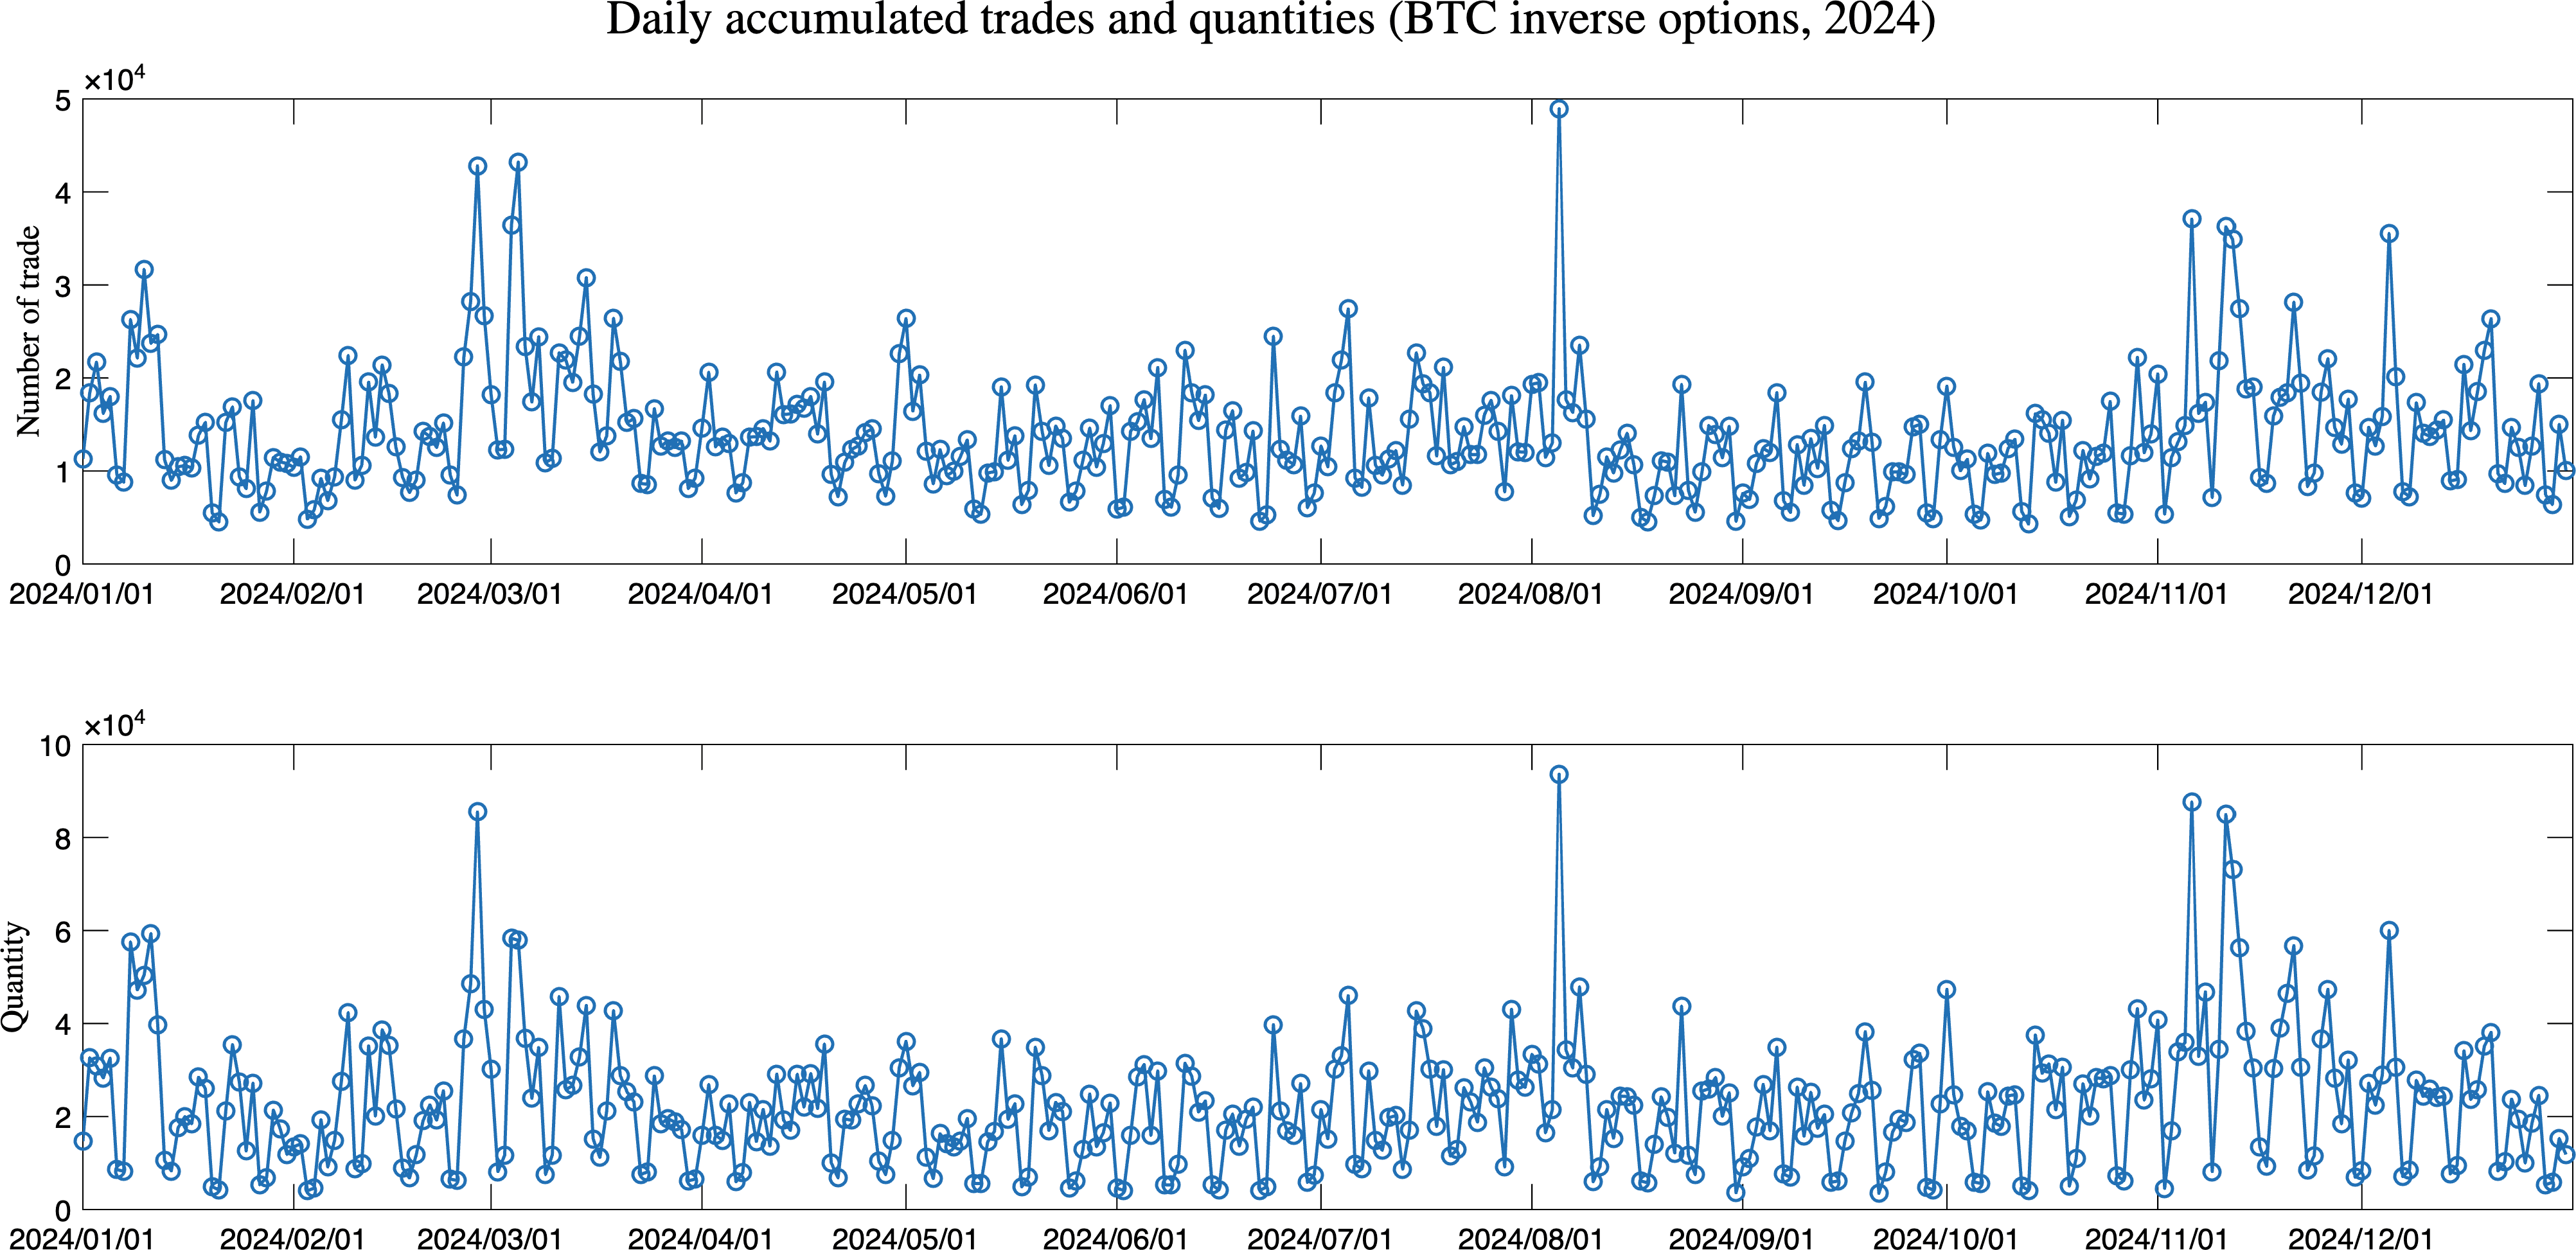
\includegraphics[width=\linewidth]{Sections/02_data_figures/Daily_traded_quantity.png}
    \caption{\textbf{Daily trading activity in the full-year intraday option sample.} The upper panel reports the daily number of BTC inverse-option trades, and the lower panel reports total daily contract quantity in 2024.}
    \label{fig:appendix_full_year_option_activity}
\end{figure}

Figure~\ref{fig:appendix_full_year_option_activity} shows daily trading activity throughout 2024, with the number of trades fluctuating between approximately 5,000 and 45,000 per day and total daily quantity ranging between 5,000 and 90,000 contracts. Two prominent spikes in both trades and quantity are visible around late February to early March and late July to early August 2024, coinciding with periods of elevated Bitcoin price volatility and heightened hedging demand.

\clearpage

\begin{figure}[h]
    \centering
    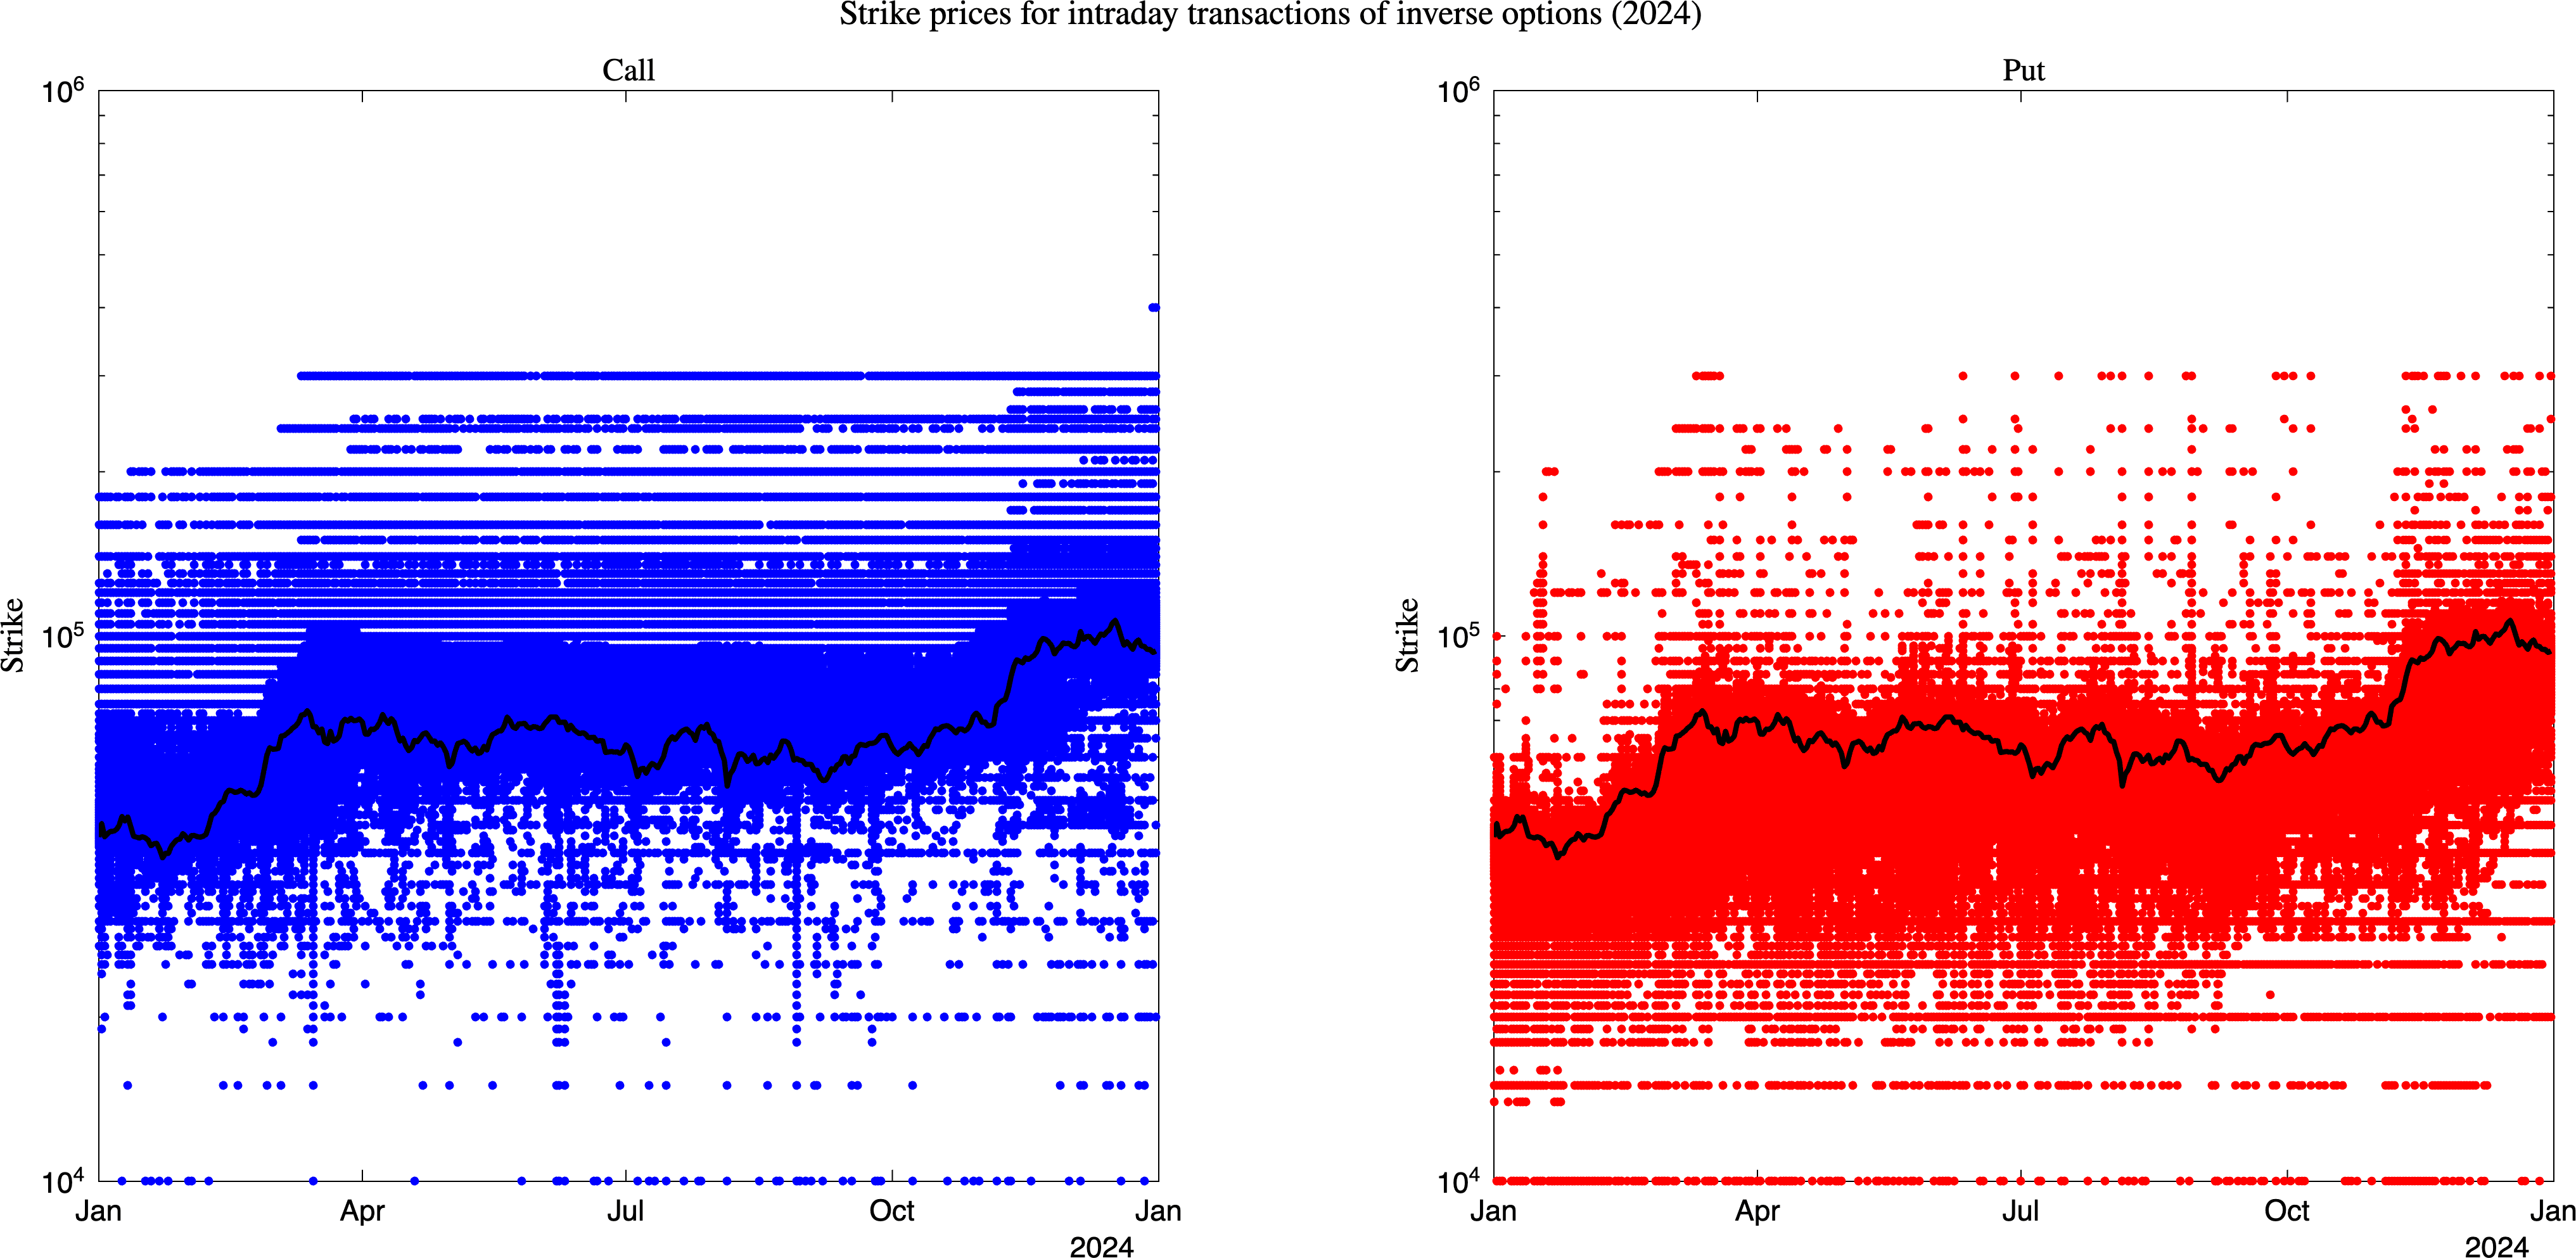
\includegraphics[width=\linewidth]{Sections/02_data_figures/Strike price for the intraday of inverse options.png}
    \caption{\textbf{Strike distribution in the full-year intraday option sample.} Calls and puts are shown separately; the black line traces the daily BTC spot-price proxy. Strike and spot prices are reported in US dollars on a logarithmic scale.}
    \label{fig:appendix_full_year_option_strikes}
\end{figure}

Figure~\ref{fig:appendix_full_year_option_strikes} illustrates the cross-sectional distribution of strike prices across the full year for calls (blue) and puts (red), with the black line tracing the daily spot price. Strikes span more than two orders of magnitude on a logarithmic scale---from approximately \$10,000 to \$1,000,000---with the densest concentration surrounding the at-the-money level. The upward drift of the strike distribution mirrors the appreciation of the underlying spot price.

\clearpage

\begin{table}[h]
\centering
\begin{tabular}{lrrrrrr}
\hline
 & \multicolumn{2}{c}{$T$} & \multicolumn{2}{c}{$S_0/K$} & \multicolumn{2}{c}{$p$} \\
 Percentile & Call & Put & Call & Put & Call & Put \\
\hline
Min & 0 & 0 & 0.17 & 0.17 & 0.0001 & 0.0001 \\
$Q_1$ & 0 & 0 & 0.45 & 0.91 & 0.0001 & 0.0001 \\
$Q_5$ & 1 & 0 & 0.68 & 0.98 & 0.0003 & 0.0003 \\
$Q_{10}$ & 1 & 1 & 0.78 & 1.00 & 0.0006 & 0.0005 \\
$Q_{20}$ & 1 & 1 & 0.87 & 1.00 & 0.0021 & 0.0015 \\
$Q_{30}$ & 2 & 2 & 0.91 & 1.01 & 0.0042 & 0.0030 \\
$Q_{40}$ & 3 & 3 & 0.94 & 1.03 & 0.0070 & 0.0050 \\
$Q_{50}$ & 7 & 4 & 0.96 & 1.04 & 0.0105 & 0.0079 \\
$Q_{60}$ & 11 & 8 & 0.97 & 1.06 & 0.0160 & 0.0115 \\
$Q_{70}$ & 18 & 14 & 0.99 & 1.09 & 0.0255 & 0.0170 \\
$Q_{80}$ & 31 & 22 & 1.00 & 1.13 & 0.0405 & 0.0270 \\
$Q_{90}$ & 65 & 50 & 1.01 & 1.22 & 0.0715 & 0.0470 \\
$Q_{95}$ & 114 & 80 & 1.04 & 1.36 & 0.1070 & 0.0720 \\
$Q_{99}$ & 283 & 215 & 1.19 & 1.97 & 0.2325 & 0.1540 \\
$Q_{99.9}$ & 354 & 343 & 2.10 & 4.71 & 0.5315 & 0.5701 \\
$Q_{99.99}$ & 364 & 363 & 4.93 & 9.00 & 0.8110 & 2.1930 \\
Max & 365 & 365 & 10.23 & 10.02 & 0.9025 & 4.8170 \\
\hline
\end{tabular}
\caption{\textbf{Distributions of full-year intraday option characteristics.} The table presents observation-weighted percentiles of time to maturity ($T$, in days), moneyness ($S_0/K$), and transaction price ($p$, in BTC) for calls and puts.}
\label{tab:appendix_full_year_option_characteristics}
\end{table}

Tables~\ref{tab:appendix_full_year_option_characteristics} and~\ref{tab:appendix_full_year_weighted_option_characteristics} report the same three characteristics---time to maturity ($T$), moneyness ($S_0/K$), and price ($p$)---but the latter reweights each observation by traded quantity. The comparison reveals a systematic shift in the bulk of the distribution once size is accounted for.

For maturity, the weighted median maturity roughly doubles relative to the unweighted median (calls: 7 $\to$ 14 days; puts: 4 $\to$ 9 days), and this pattern persists through the 90th percentile (calls: 65 $\to$ 98; puts: 50 $\to$ 65). This indicates that larger trades are disproportionately concentrated in longer-dated contracts, rather than in the very short-dated options that dominate the raw contract count.

For moneyness, volume-weighting pulls the put-side distribution further out-of-the-money - the $Q_{90}$ for puts rises from 1.22 to 1.29 and $Q_{95}$
from 1.36 to 1.45 - while the call side is little changed or slightly more concentrated near-the-money at the median (0.96 $\to$ 0.93). This asymmetry is consistent with large-size trading activity being driven by downside/tail-hedging demand rather than symmetric directional speculation.

For price, reflecting both the longer maturities and deeper OTM put skew, weighted median prices are noticeably higher (calls: 0.0105 $\to$ 0.0162; puts: 0.0079 $\to$ 0.0105 BTC).

Notably, the extreme upper tail ($Q_{99.9}$ and beyond) is nearly identical across both tables for all three characteristics, since these percentiles are anchored by the same small set of extreme contracts regardless of weighting. The divergence is therefore a genuine feature of the bulk of the distribution, not an artifact of outliers - a useful diagnostic if you weight your Q-calibration loss function by trade size, since doing so will implicitly shift emphasis toward longer-dated, more OTM put contracts relative to an unweighted (per-contract) loss.

\begin{table}[h]
\centering
\begin{tabular}{lrrrrrr}
\hline
 & \multicolumn{2}{c}{$T$} & \multicolumn{2}{c}{$S_0/K$} & \multicolumn{2}{c}{$p$} \\
 Percentile & Call & Put & Call & Put & Call & Put \\
\hline
Min & 0 & 0 & 0.17 & 0.17 & 0.0001 & 0.0001 \\
$Q_1$ & 0 & 0 & 0.42 & 0.91 & 0.0001 & 0.0001 \\
$Q_5$ & 1 & 1 & 0.61 & 0.98 & 0.0005 & 0.0004 \\
$Q_{10}$ & 1 & 1 & 0.70 & 1.00 & 0.0015 & 0.0009 \\
$Q_{20}$ & 2 & 2 & 0.81 & 1.01 & 0.0042 & 0.0025 \\
$Q_{30}$ & 5 & 3 & 0.87 & 1.02 & 0.0075 & 0.0047 \\
$Q_{40}$ & 9 & 7 & 0.91 & 1.04 & 0.0110 & 0.0073 \\
$Q_{50}$ & 14 & 9 & 0.93 & 1.06 & 0.0162 & 0.0105 \\
$Q_{60}$ & 21 & 14 & 0.96 & 1.08 & 0.0235 & 0.0150 \\
$Q_{70}$ & 35 & 21 & 0.97 & 1.12 & 0.0340 & 0.0212 \\
$Q_{80}$ & 53 & 36 & 0.99 & 1.18 & 0.0505 & 0.0315 \\
$Q_{90}$ & 98 & 65 & 1.00 & 1.29 & 0.0829 & 0.0535 \\
$Q_{95}$ & 162 & 102 & 1.04 & 1.45 & 0.1210 & 0.0786 \\
$Q_{99}$ & 273 & 226 & 1.23 & 2.21 & 0.2388 & 0.1520 \\
$Q_{99.9}$ & 354 & 337 & 1.96 & 7.08 & 0.5075 & 0.3670 \\
$Q_{99.99}$ & 364 & 363 & 3.52 & 9.71 & 0.7320 & 1.6420 \\
Max & 365 & 365 & 10.23 & 10.02 & 0.9025 & 4.8170 \\
\hline
\end{tabular}
\caption{\textbf{Quantity-weighted distributions of full-year intraday option characteristics.} The table presents transaction-quantity-weighted percentiles of time to maturity ($T$, in days), moneyness ($S_0/K$), and transaction price ($p$, in BTC).}
\label{tab:appendix_full_year_weighted_option_characteristics}
\end{table}



\clearpage

\begin{table}[h]
\centering
\begin{tabular}{lrrrr}
\hline
Inverse BTC call option & Deep OTM & OTM & ITM & \\
 & $\frac{S_0}{K} \leq 0.86$ & $0.86 < \frac{S_0}{K} \leq 1$ & $1 < \frac{S_0}{K}$ & Sum \\
\hline
Short-term: $T \leq 7$ & 0.8\% & 23.4\% & 4.4\% & 28.6\% \\
Mid-term: $7 < T \leq 28$ & 2.8\% & 9.4\% & 2.4\% & 14.7\% \\
Long-term: $28 < T$ & 6.4\% & 4.0\% & 1.3\% & 11.8\% \\
Sum & 10.0\% & 36.9\% & 8.2\% & 55.1\% \\
\hline
Inverse BTC put option & ITM & OTM & Deep OTM & \\
 & $\frac{S_0}{K} \leq 1$ & $1 < \frac{S_0}{K} \leq 1.12$ &  $1.12 < \frac{S_0}{K}$ & Sum \\
\hline
Short-term: $T \leq 7$ & 3.5\% & 20.4\% & 2.2\% & 26.1\% \\
Mid-term: $7 < T \leq 28$ & 1.4\% & 6.2\% & 3.4\% & 11.1\% \\
Long-term: $28 < T$ & 1.3\% & 2.3\% & 4.2\% & 7.7\% \\
Sum & 6.2\% & 29.0\% & 9.8\% & 44.9\% \\
\hline
\end{tabular}
\caption{\textbf{Maturity--moneyness composition of the full-year intraday sample.} The table reports the percentage of transactions in each maturity--moneyness category.}
\label{tab:appendix_full_year_maturity_moneyness}

\end{table}

Tables~\ref{tab:appendix_full_year_maturity_moneyness} and~\ref{tab:appendix_full_year_weighted_maturity_moneyness} partition trading activity into a 3$\times$3 maturity--moneyness grid for calls and puts separately, contrasting the raw trade-count distribution with the quantity-weighted distribution. Two consistent patterns emerge once volume is used as the weight instead of trade count.

Shift from short-term to long-term. Under the unweighted count, short-term options ($T\le 7$) dominate both calls (28.6\%) and puts (26.1\%), while long-term options are the smallest bucket (11.8\% calls, 7.7\% puts). Weighting by quantity essentially reverses this ordering for calls: long-term rises to 20.5\%, roughly matching short-term's 21.7\%, while for puts the short-term share falls (26.1\% to 17.6\%) and the long-term share rises (7.7\% to 9.7\%). This confirms what Table~\ref{tab:appendix_full_year_weighted_option_characteristics} suggests from the marginal maturity distribution: larger full-day trades cluster in longer-dated contracts.

Shift toward deep OTM, especially at long maturities. The clearest movement is in the OTM/deep-OTM composition. For calls, deep-OTM share more than doubles for the long-term bucket alone (6.4\% $\to$ 12.4\%), and the overall call deep-OTM sum rises from 10.0\% to 17.1\%. For puts, the deep-OTM long-term cell rises from 4.2\% to 5.6\%, and overall put deep-OTM rises from 9.8\% to 11.8\%, while the near-the-money OTM bucket shrinks correspondingly (put OTM sum: 29.0\% → 22.6\%). This is consistent with the earlier percentile analysis: large trades skew toward tail hedges rather than near-the-money speculative flow.

Calls vs. puts asymmetry persists. Across both weighting schemes, calls retain a higher overall trading share than puts (55.1\% vs. 44.9\% unweighted; 60.6\% vs. 39.4\% weighted), and this gap widens under volume weighting — implying call-side activity is not just more frequent but carried out in larger size, plausibly reflecting basis-trade or covered-call-type flow that's naturally larger in inverse (BTC-margined) contracts.


\begin{table}[h]
\centering
\begin{tabular}{lrrrr}
\hline
Inverse BTC call option & Deep OTM & OTM & ITM & \\
 & $\frac{S_0}{K} \leq 0.86$ & $0.86 < \frac{S_0}{K} \leq 1$ & $1 < \frac{S_0}{K}$ & Sum \\
\hline
Short-term: $T \leq 7$ & 1.0\% & 17.5\% & 3.2\% & 21.7\% \\
Mid-term: $7 < T \leq 28$ & 3.8\% & 12.4\% & 2.4\% & 18.5\% \\
Long-term: $28 < T$ & 12.4\% & 6.2\% & 1.9\% & 20.5\% \\
Sum & 17.1\% & 36.1\% & 7.4\% & 60.6\% \\
\hline
Inverse BTC put option & ITM & OTM & Deep OTM & \\
 & $\frac{S_0}{K} \leq 1$ & $1 < \frac{S_0}{K} \leq 1.12$ &  $1.12 < \frac{S_0}{K}$ & Sum \\
\hline
Short-term: $T \leq 7$ & 2.3\% & 13.2\% & 2.0\% & 17.6\% \\
Mid-term: $7 < T \leq 28$ & 1.4\% & 6.5\% & 4.2\% & 12.1\% \\
Long-term: $28 < T$ & 1.3\% & 2.8\% & 5.6\% & 9.7\% \\
Sum & 5.0\% & 22.6\% & 11.8\% & 39.4\% \\
\hline
\end{tabular}
\caption{\textbf{Quantity-weighted maturity--moneyness composition of the full-year intraday sample.} The table reports each category's percentage of total transaction quantity.}
\label{tab:appendix_full_year_weighted_maturity_moneyness}
\end{table}


\clearpage


\begin{table}[h]
\centering

\begin{tabular}{lccc}
\hline
Inverse BTC call option & Deep OTM & OTM & ITM  \\
 & $\frac{S_0}{K} \leq 0.86$ & $0.86 < \frac{S_0}{K} \leq 1$ & $1 < \frac{S_0}{K}$  \\
\hline
Short-term: $T \leq 7$ & \makecell{0.0008\\(0.0011)} & \makecell{0.0055\\(0.0061)} & \makecell{0.0326\\(0.0451)} \\
Mid-term: $7 < T \leq 28$ & \makecell{0.0053\\(0.0050)} & \makecell{0.0231\\(0.0145)} & \makecell{0.0905\\(0.0830)} \\
Long-term: $28 < T$ & \makecell{0.0374\\(0.0414)} & \makecell{0.0782\\(0.0461)} & \makecell{0.1873\\(0.1243)} \\
\hline
Inverse BTC put option & ITM & OTM & Deep OTM \\
 & $\frac{S_0}{K} \leq 1$ & $1 < \frac{S_0}{K} \leq 1.12$ &  $1.12 < \frac{S_0}{K}$ \\
\hline
Short-term: $T \leq 7$ & \makecell{0.0252\\(0.0319)} & \makecell{0.0053\\(0.0057)} & \makecell{0.0011\\(0.0015)} \\
Mid-term: $7 < T \leq 28$ & \makecell{0.0641\\(0.0569)} & \makecell{0.0220\\(0.0120)} & \makecell{0.0052\\(0.0044)} \\
Long-term: $28 < T$ & \makecell{0.1761\\(0.2642)} & \makecell{0.0594\\(0.0275)} & \makecell{0.0202\\(0.0200)} \\
\hline
\end{tabular}
\caption{\textbf{Option prices across maturity--moneyness categories in the full-year intraday sample.} Cells report mean transaction prices in BTC, with standard deviations in parentheses.}
\label{tab:appendix_full_year_option_prices}
\end{table}

\begin{table}
\centering

\begin{tabular}{lccc}
\hline
Inverse BTC call option & Deep OTM & OTM & ITM  \\
 & $\frac{S_0}{K} \leq 0.86$ & $0.86 < \frac{S_0}{K} \leq 1$ & $1 < \frac{S_0}{K}$  \\
\hline
Short-term: $T \leq 7$ & \makecell{0.0007\\(0.0011)} & \makecell{0.0069\\(0.0068)} & \makecell{0.0415\\(0.0522)} \\
Mid-term: $7 < T \leq 28$ & \makecell{0.0058\\(0.0055)} & \makecell{0.0230\\(0.0143)} & \makecell{0.0968\\(0.0849)} \\
Long-term: $28 < T$ & \makecell{0.0369\\(0.0371)} & \makecell{0.0726\\(0.0413)} & \makecell{0.1787\\(0.1067)} \\
\hline
Inverse BTC put option & ITM & OTM & Deep OTM \\
 & $\frac{S_0}{K} \leq 1$ & $1 < \frac{S_0}{K} \leq 1.12$ &  $1.12 < \frac{S_0}{K}$ \\
\hline
Short-term: $T \leq 7$ & \makecell{0.0292\\(0.0369)} & \makecell{0.0067\\(0.0064)} & \makecell{0.0013\\(0.0017)} \\
Mid-term: $7 < T \leq 28$ & \makecell{0.0649\\(0.0507)} & \makecell{0.0212\\(0.0118)} & \makecell{0.0053\\(0.0046)} \\
Long-term: $28 < T$ & \makecell{0.1366\\(0.1660)} & \makecell{0.0566\\(0.0276)} & \makecell{0.0205\\(0.0193)} \\
\hline
\end{tabular}
\caption{\textbf{Quantity-weighted option prices across maturity--moneyness categories in the full-year intraday sample.} Cells report quantity-weighted mean transaction prices in BTC, with weighted standard deviations in parentheses.}
\label{tab:appendix_full_year_weighted_option_prices}
\end{table}

Tables~\ref{tab:appendix_full_year_option_prices} and~\ref{tab:appendix_full_year_weighted_option_prices} report mean BTC-denominated prices (with standard deviations) across the same nine maturity--moneyness buckets, unweighted per observation versus weighted by traded quantity. Three patterns stand out.

Monotonicity confirms internal consistency. Within both tables, prices rise monotonically with maturity for every moneyness bucket (as expected from time value), and rise monotonically with moneyness for calls (deep OTM cheapest, ITM most expensive) while falling monotonically with moneyness for puts. This is a useful sanity check: the data respects basic no-arbitrage ordering before any model fitting is applied, so any monotonicity violations you find later in the pricing kernel estimate can't be traced back to a raw data pathology at this level.

Weighting effects are asymmetric and bucket-specific, not uniform. Rather than a systematic upward or downward shift, quantity weighting moves prices in different directions depending on the cell. Short-term ITM calls are notably more expensive when weighted (0.0326 to 0.0415), whereas long-term ITM puts are substantially cheaper (0.1761 to 0.1366) and long-term ITM calls are slightly cheaper (0.1873 to 0.1787). A uniform ``volume-weighting effect'' therefore cannot be assumed across the calibration grid.

Dispersion is high in several long-term buckets. Long-term ITM puts, for example, have an unweighted standard deviation of 0.2642 BTC, exceeding their mean of 0.1761 BTC. This heterogeneity cautions against interpreting a category average as a single contemporaneous option surface, which is one reason the main analysis uses the narrow closing window described in Section~\ref{subsec:deribit_filtered_options}.
\clearpage
    \subsection*{What is Bayesian Inference?}
Bayesian inference is a statistical framework for updating beliefs about
unknown quantities in light of observed data. Unlike the frequentist
approach, which treats parameters as fixed but unknown constants, Bayesian
inference treats the parameter vector $\bm{\Theta}$ (in the SVCJ setting,
the parameters $\kappa, \theta, \sigma_v, \rho, \lambda$, and the
jump-related terms) as a random variable with its own probability
distribution.
 
The framework rests on Bayes' theorem:
\begin{equation}
    p(\bm{\Theta} \mid y) = \frac{p(y \mid \bm{\Theta})\,p(\bm{\Theta})}{p(y)}
    \propto p(y \mid \bm{\Theta})\,p(\bm{\Theta})
    \label{eq:bayes}
\end{equation}
where $y$ denotes the observed data (daily Bitcoin returns). Three objects
matter here:
 
\begin{itemize}
    \item \textbf{Prior}, $p(\bm{\Theta})$ --- the belief about $\bm{\Theta}$
    before observing any data, specified by the researcher.
    \item \textbf{Likelihood}, $p(y \mid \bm{\Theta})$ --- the probability of
    observing the data given a particular value of $\bm{\Theta}$, determined
    by the SVCJ model's dynamics.
    \item \textbf{Posterior}, $p(\bm{\Theta} \mid y)$ --- the updated belief
    about $\bm{\Theta}$ after observing the data, and the actual object of
    inference.
\end{itemize}
 
The normalizing constant $p(y)$ does not depend on $\bm{\Theta}$ and can be
dropped in the proportionality in \eqref{eq:bayes}; this becomes important
in Section~\ref{sec:mcmc}.
 
In the SVCJ setting, Bayesian inference means estimating the entire
posterior distribution of the parameters and the latent variance path
$V_t$, rather than a single point estimate --- giving not just parameter
values but a full characterization of estimation uncertainty (e.g.,
credible intervals), which is valuable when addressing the pricing kernel
puzzle.
\clearpage

\subsection*{Why MCMC Works: Stationarity, Detailed Balance, and a Discrete Example}
\label{subsec:mcmc_theory}

The preceding subsection describes what the Metropolis--Hastings recipe does.
This subsection states why it is valid: why a chain constructed from
unnormalized density ratios reproduces the correct posterior, and at what rate
it does so. A three-state example makes every quantity explicit.

\subsubsection*{Stationarity}

Let $\pi$ denote the target distribution --- here the posterior
$p(\bm{\Theta}\mid y)$ --- known only up to the normalizing constant
\eqref{eq:normconst}, so that $\pi(x)\propto w(x)$ for a computable weight
function $w$. A Markov chain on a state space $\mathcal{X}$ is characterized by
its transition kernel
\begin{equation}
    P(x,y)=\Pr\left(X_{t+1}=y \mid X_t=x\right),
    \qquad \sum_{y\in\mathcal{X}}P(x,y)=1,
    \label{eq:kernel}
\end{equation}
and a distribution evolves according to $\mu_{t+1}=\mu_t P$. The distribution
$\pi$ is \emph{stationary} for $P$ if
\begin{equation}
    \pi P=\pi,
    \qquad\text{that is,}\qquad
    \sum_{x\in\mathcal{X}}\pi(x)P(x,y)=\pi(y)
    \quad\text{for all }y\in\mathcal{X}.
    \label{eq:stationary}
\end{equation}
Once the marginal law of the chain equals $\pi$, it remains $\pi$ at every
subsequent step. Condition \eqref{eq:stationary} is global---it couples every
state to every other---and is therefore awkward to impose directly when
designing an algorithm.

\subsubsection*{Detailed balance}

The practical route is to impose a stronger but purely \emph{pairwise}
condition. The chain is \emph{reversible} with respect to $\pi$, equivalently
satisfies \emph{detailed balance}, if
\begin{equation}
    \pi(x)P(x,y)=\pi(y)P(y,x)
    \qquad\text{for all }x,y\in\mathcal{X}.
    \label{eq:detailed_balance}
\end{equation}
Read as a statement about flows, \eqref{eq:detailed_balance} requires the
probability mass moving from $x$ to $y$ in stationarity to equal the mass
moving from $y$ to $x$.

\begin{proposition}
Detailed balance \eqref{eq:detailed_balance} implies stationarity
\eqref{eq:stationary}.
\label{prop:db_implies_stationarity}
\end{proposition}

\begin{proof}
Summing \eqref{eq:detailed_balance} over $x$ and using $\sum_{x}P(y,x)=1$,
\begin{equation*}
    \sum_{x}\pi(x)P(x,y)
    =\sum_{x}\pi(y)P(y,x)
    =\pi(y)\sum_{x}P(y,x)
    =\pi(y),
\end{equation*}
which is precisely \eqref{eq:stationary}.
\end{proof}

Proposition~\ref{prop:db_implies_stationarity} is the design principle behind
every Metropolis--Hastings sampler: a condition that can be verified one pair of
states at a time delivers the global fixed-point property that is actually
required. The converse does not hold---a stationary chain need not be
reversible---but reversible chains are far easier to construct.

\subsubsection*{Convergence and the ergodic theorem}

Stationarity alone does not guarantee that the chain \emph{reaches} $\pi$ from
an arbitrary starting point. Two further conditions are needed. The chain is
\emph{irreducible} if every state is reachable from every other in finitely many
steps, and \emph{aperiodic} if it is not confined to a deterministic cycle.
Under irreducibility and aperiodicity, for any initial distribution $\mu_0$,
\begin{equation}
    \left\|\mu_0P^{t}-\pi\right\|_{TV}\longrightarrow 0
    \qquad\text{and}\qquad
    \frac{1}{T}\sum_{t=1}^{T}f\left(X_t\right)
    \xrightarrow{\text{ a.s. }}\mathbb{E}_{\pi}\left[f\right]
    \label{eq:ergodic}
\end{equation}
for every $\pi$-integrable $f$. The second statement is the ergodic theorem. It
is the law of large numbers for dependent draws, and it is what licenses
estimating posterior means and quantiles by averaging along a single realized
chain.

\subsubsection*{Metropolis--Hastings satisfies detailed balance}

\begin{proposition}
Let $q(x,\cdot)$ be any proposal kernel and let
\begin{equation}
    \alpha(x,y)=\min\left\{1,\ \frac{w(y)\,q(y,x)}{w(x)\,q(x,y)}\right\}
    \label{eq:mh_general}
\end{equation}
be the associated acceptance probability. Then the chain with off-diagonal
kernel $P(x,y)=q(x,y)\alpha(x,y)$ for $y\neq x$, and with the residual mass
placed on $P(x,x)$, satisfies detailed balance \eqref{eq:detailed_balance} with
respect to $\pi\propto w$.
\label{prop:mh_db}
\end{proposition}

\begin{proof}
Fix $x\neq y$ and suppose without loss of generality that
$w(y)q(y,x)\leq w(x)q(x,y)$, so that
$\alpha(x,y)=w(y)q(y,x)/\left[w(x)q(x,y)\right]$ and $\alpha(y,x)=1$. Then
\begin{equation*}
    \pi(x)P(x,y)
    \propto w(x)\,q(x,y)\,\frac{w(y)\,q(y,x)}{w(x)\,q(x,y)}
    =w(y)\,q(y,x)
    =w(y)\,q(y,x)\,\alpha(y,x)
    \propto \pi(y)P(y,x).
\end{equation*}
The reverse inequality follows by symmetry, and the case $x=y$ is immediate.
\end{proof}

Only the ratio $w(y)/w(x)$ enters \eqref{eq:mh_general}. The normalizing
constant \eqref{eq:normconst} cancels, which is the property already exploited
in \eqref{eq:mh}. Combining Propositions~\ref{prop:db_implies_stationarity}
and~\ref{prop:mh_db} with \eqref{eq:ergodic} completes the justification: the
sampler targets $\pi$, and time averages along its path converge to posterior
expectations.

\subsubsection*{A three-state example}

Let $\mathcal{X}=\{1,2,3\}$ and suppose only the unnormalized weights
\begin{equation*}
    w(1)=1,\qquad w(2)=2,\qquad w(3)=3
\end{equation*}
can be evaluated, the constant $w(1)+w(2)+w(3)=6$ being treated as unknown
exactly as $p(y)$ is unknown in \eqref{eq:normconst}. The target is therefore
$\pi=\left(\tfrac{1}{6},\tfrac{1}{3},\tfrac{1}{2}\right)$, which the algorithm
must recover without ever using the number $6$.

Take the symmetric proposal that moves to one of the two other states with equal
probability, $q(x,y)=\tfrac{1}{2}$ for $y\neq x$. The proposal terms in
\eqref{eq:mh_general} cancel, leaving $\alpha(x,y)=\min\{1,w(y)/w(x)\}$. From
state $2$, for instance,
\begin{equation*}
    P(2,1)=\tfrac{1}{2}\min\left\{1,\tfrac{1}{2}\right\}=\tfrac{1}{4},
    \qquad
    P(2,3)=\tfrac{1}{2}\min\left\{1,\tfrac{3}{2}\right\}=\tfrac{1}{2},
\end{equation*}
with the remaining mass $P(2,2)=1-\tfrac{1}{4}-\tfrac{1}{2}=\tfrac{1}{4}$
assigned to the rejection event, in which the chain stays where it is. Note that
moves toward higher weight are always accepted, while moves toward lower weight
are accepted in proportion to the weight ratio. Collecting all three rows,
\begin{equation}
    P=\begin{pmatrix}
        0 & 1/2 & 1/2\\
        1/4 & 1/4 & 1/2\\
        1/6 & 1/3 & 1/2
    \end{pmatrix}.
    \label{eq:toy_kernel}
\end{equation}

Detailed balance \eqref{eq:detailed_balance} may be verified one pair at a time:

\begin{center}
\begin{tabular}{ccc}
\toprule
$(x,y)$ & $\pi(x)P(x,y)$ & $\pi(y)P(y,x)$\\
\midrule
$(1,2)$ & $\tfrac{1}{6}\cdot\tfrac{1}{2}=\tfrac{1}{12}$
        & $\tfrac{1}{3}\cdot\tfrac{1}{4}=\tfrac{1}{12}$\\
$(1,3)$ & $\tfrac{1}{6}\cdot\tfrac{1}{2}=\tfrac{1}{12}$
        & $\tfrac{1}{2}\cdot\tfrac{1}{6}=\tfrac{1}{12}$\\
$(2,3)$ & $\tfrac{1}{3}\cdot\tfrac{1}{2}=\tfrac{1}{6}$
        & $\tfrac{1}{2}\cdot\tfrac{1}{3}=\tfrac{1}{6}$\\
\bottomrule
\end{tabular}
\end{center}

By Proposition~\ref{prop:db_implies_stationarity}, $\pi$ is stationary for
\eqref{eq:toy_kernel}. Starting the chain deterministically in state $1$, so
that $\mu_0=(1,0,0)$, the marginal distribution evolves as follows.

\begin{center}
\begin{tabular}{cccc}
\toprule
$t$ & $\mu_t(1)$ & $\mu_t(2)$ & $\mu_t(3)$\\
\midrule
$0$ & $1.0000$ & $0.0000$ & $0.0000$\\
$1$ & $0.0000$ & $0.5000$ & $0.5000$\\
$2$ & $0.2083$ & $0.2917$ & $0.5000$\\
$3$ & $0.1563$ & $0.3438$ & $0.5000$\\
$4$ & $0.1693$ & $0.3307$ & $0.5000$\\
\midrule
$\pi$ & $0.1667$ & $0.3333$ & $0.5000$\\
\bottomrule
\end{tabular}
\end{center}

The error in the first coordinate equals $\tfrac{1}{24}$, $-\tfrac{1}{96}$ and
$\tfrac{1}{384}$ at $t=2,3,4$: it contracts by a factor of four and alternates
in sign at each step. That factor is the second-largest eigenvalue of
\eqref{eq:toy_kernel} in modulus, $\lambda_2=-1/4$. In general
\begin{equation}
    \left\|\mu_t-\pi\right\|_{TV}=O\left(\left|\lambda_2\right|^{t}\right),
    \label{eq:spectral}
\end{equation}
so the \emph{spectral gap} $1-\left|\lambda_2\right|$ governs the rate of
convergence; a chain that mixes slowly is one whose spectral gap is close to
zero.

The construction used only the ratios $w(2)/w(1)=2$, $w(3)/w(1)=3$ and
$w(3)/w(2)=3/2$. The normalizing constant never appeared, yet the chain
reproduces $\pi$ exactly. With three states one would of course normalize
directly and sample without recourse to MCMC. The value of the argument is that
nothing in it depends on the cardinality of $\mathcal{X}$: Propositions
\ref{prop:db_implies_stationarity} and \ref{prop:mh_db} apply verbatim when the
state is the parameter vector $\bm{\Theta}$ together with the latent variance
path $\left\{V_t\right\}$, where \eqref{eq:normconst} is unavailable but the
weight ratios remain elementary to compute.

\subsubsection*{Practical consequences}

Three implications for the estimation under $\mathbb{P}$ follow directly from
\eqref{eq:ergodic} and \eqref{eq:spectral}.

First, the convergence in \eqref{eq:ergodic} is asymptotic. Draws generated
before the chain has approached $\pi$ still carry the influence of $\mu_0$ and
are discarded as burn-in.

Second, consecutive draws are dependent by construction. For an estimator
$\bar{f}_T=T^{-1}\sum_{t=1}^{T}f\left(X_t\right)$ the relevant sample size is
not $T$ but the effective sample size
\begin{equation}
    \mathrm{ESS}=\frac{T}{1+2\sum_{k=1}^{\infty}\rho_k},
    \label{eq:ess}
\end{equation}
where $\rho_k$ denotes the lag-$k$ autocorrelation of
$\left\{f\left(X_t\right)\right\}$. A slowly mixing chain can produce $T=10^{5}$
draws whose information content is equivalent to only a few hundred independent
ones.

Third, the proposal scale is a genuine tuning parameter. Proposals that are too
narrow are almost always accepted but explore the state space slowly, while
proposals that are too wide are almost always rejected. Neither pathology
violates \eqref{eq:ergodic}, but both inflate \eqref{eq:ess}. Convergence is
therefore assessed empirically---through trace plots, autocorrelation functions,
and the comparison of within- and between-chain variance across dispersed
starting values---rather than being assumed.



\end{document}
